% Options for packages loaded elsewhere
\PassOptionsToPackage{unicode}{hyperref}
\PassOptionsToPackage{hyphens}{url}
%
\documentclass[
]{book}
\usepackage{amsmath,amssymb}
\usepackage{lmodern}
\usepackage{ifxetex,ifluatex}
\ifnum 0\ifxetex 1\fi\ifluatex 1\fi=0 % if pdftex
  \usepackage[T1]{fontenc}
  \usepackage[utf8]{inputenc}
  \usepackage{textcomp} % provide euro and other symbols
\else % if luatex or xetex
  \usepackage{unicode-math}
  \defaultfontfeatures{Scale=MatchLowercase}
  \defaultfontfeatures[\rmfamily]{Ligatures=TeX,Scale=1}
\fi
% Use upquote if available, for straight quotes in verbatim environments
\IfFileExists{upquote.sty}{\usepackage{upquote}}{}
\IfFileExists{microtype.sty}{% use microtype if available
  \usepackage[]{microtype}
  \UseMicrotypeSet[protrusion]{basicmath} % disable protrusion for tt fonts
}{}
\makeatletter
\@ifundefined{KOMAClassName}{% if non-KOMA class
  \IfFileExists{parskip.sty}{%
    \usepackage{parskip}
  }{% else
    \setlength{\parindent}{0pt}
    \setlength{\parskip}{6pt plus 2pt minus 1pt}}
}{% if KOMA class
  \KOMAoptions{parskip=half}}
\makeatother
\usepackage{xcolor}
\IfFileExists{xurl.sty}{\usepackage{xurl}}{} % add URL line breaks if available
\IfFileExists{bookmark.sty}{\usepackage{bookmark}}{\usepackage{hyperref}}
\hypersetup{
  pdftitle={Test},
  pdfauthor={Prepared by the EUROCONTROL Performance Review Unit (PRU)},
  hidelinks,
  pdfcreator={LaTeX via pandoc}}
\urlstyle{same} % disable monospaced font for URLs
\usepackage{color}
\usepackage{fancyvrb}
\newcommand{\VerbBar}{|}
\newcommand{\VERB}{\Verb[commandchars=\\\{\}]}
\DefineVerbatimEnvironment{Highlighting}{Verbatim}{commandchars=\\\{\}}
% Add ',fontsize=\small' for more characters per line
\usepackage{framed}
\definecolor{shadecolor}{RGB}{248,248,248}
\newenvironment{Shaded}{\begin{snugshade}}{\end{snugshade}}
\newcommand{\AlertTok}[1]{\textcolor[rgb]{0.94,0.16,0.16}{#1}}
\newcommand{\AnnotationTok}[1]{\textcolor[rgb]{0.56,0.35,0.01}{\textbf{\textit{#1}}}}
\newcommand{\AttributeTok}[1]{\textcolor[rgb]{0.77,0.63,0.00}{#1}}
\newcommand{\BaseNTok}[1]{\textcolor[rgb]{0.00,0.00,0.81}{#1}}
\newcommand{\BuiltInTok}[1]{#1}
\newcommand{\CharTok}[1]{\textcolor[rgb]{0.31,0.60,0.02}{#1}}
\newcommand{\CommentTok}[1]{\textcolor[rgb]{0.56,0.35,0.01}{\textit{#1}}}
\newcommand{\CommentVarTok}[1]{\textcolor[rgb]{0.56,0.35,0.01}{\textbf{\textit{#1}}}}
\newcommand{\ConstantTok}[1]{\textcolor[rgb]{0.00,0.00,0.00}{#1}}
\newcommand{\ControlFlowTok}[1]{\textcolor[rgb]{0.13,0.29,0.53}{\textbf{#1}}}
\newcommand{\DataTypeTok}[1]{\textcolor[rgb]{0.13,0.29,0.53}{#1}}
\newcommand{\DecValTok}[1]{\textcolor[rgb]{0.00,0.00,0.81}{#1}}
\newcommand{\DocumentationTok}[1]{\textcolor[rgb]{0.56,0.35,0.01}{\textbf{\textit{#1}}}}
\newcommand{\ErrorTok}[1]{\textcolor[rgb]{0.64,0.00,0.00}{\textbf{#1}}}
\newcommand{\ExtensionTok}[1]{#1}
\newcommand{\FloatTok}[1]{\textcolor[rgb]{0.00,0.00,0.81}{#1}}
\newcommand{\FunctionTok}[1]{\textcolor[rgb]{0.00,0.00,0.00}{#1}}
\newcommand{\ImportTok}[1]{#1}
\newcommand{\InformationTok}[1]{\textcolor[rgb]{0.56,0.35,0.01}{\textbf{\textit{#1}}}}
\newcommand{\KeywordTok}[1]{\textcolor[rgb]{0.13,0.29,0.53}{\textbf{#1}}}
\newcommand{\NormalTok}[1]{#1}
\newcommand{\OperatorTok}[1]{\textcolor[rgb]{0.81,0.36,0.00}{\textbf{#1}}}
\newcommand{\OtherTok}[1]{\textcolor[rgb]{0.56,0.35,0.01}{#1}}
\newcommand{\PreprocessorTok}[1]{\textcolor[rgb]{0.56,0.35,0.01}{\textit{#1}}}
\newcommand{\RegionMarkerTok}[1]{#1}
\newcommand{\SpecialCharTok}[1]{\textcolor[rgb]{0.00,0.00,0.00}{#1}}
\newcommand{\SpecialStringTok}[1]{\textcolor[rgb]{0.31,0.60,0.02}{#1}}
\newcommand{\StringTok}[1]{\textcolor[rgb]{0.31,0.60,0.02}{#1}}
\newcommand{\VariableTok}[1]{\textcolor[rgb]{0.00,0.00,0.00}{#1}}
\newcommand{\VerbatimStringTok}[1]{\textcolor[rgb]{0.31,0.60,0.02}{#1}}
\newcommand{\WarningTok}[1]{\textcolor[rgb]{0.56,0.35,0.01}{\textbf{\textit{#1}}}}
\usepackage{longtable,booktabs,array}
\usepackage{calc} % for calculating minipage widths
% Correct order of tables after \paragraph or \subparagraph
\usepackage{etoolbox}
\makeatletter
\patchcmd\longtable{\par}{\if@noskipsec\mbox{}\fi\par}{}{}
\makeatother
% Allow footnotes in longtable head/foot
\IfFileExists{footnotehyper.sty}{\usepackage{footnotehyper}}{\usepackage{footnote}}
\makesavenoteenv{longtable}
\usepackage{graphicx}
\makeatletter
\def\maxwidth{\ifdim\Gin@nat@width>\linewidth\linewidth\else\Gin@nat@width\fi}
\def\maxheight{\ifdim\Gin@nat@height>\textheight\textheight\else\Gin@nat@height\fi}
\makeatother
% Scale images if necessary, so that they will not overflow the page
% margins by default, and it is still possible to overwrite the defaults
% using explicit options in \includegraphics[width, height, ...]{}
\setkeys{Gin}{width=\maxwidth,height=\maxheight,keepaspectratio}
% Set default figure placement to htbp
\makeatletter
\def\fps@figure{htbp}
\makeatother
\setlength{\emergencystretch}{3em} % prevent overfull lines
\providecommand{\tightlist}{%
  \setlength{\itemsep}{0pt}\setlength{\parskip}{0pt}}
\setcounter{secnumdepth}{5}
\usepackage{booktabs}
\ifluatex
  \usepackage{selnolig}  % disable illegal ligatures
\fi
\usepackage[]{natbib}
\bibliographystyle{apalike}

\title{Test}
\author{Prepared by the EUROCONTROL Performance Review Unit (PRU)}
\date{December 2020}

\begin{document}
\maketitle

{
\setcounter{tocdepth}{1}
\tableofcontents
}
\hypertarget{introduction}{%
\chapter{Introduction}\label{introduction}}

The ACE benchmarking work is carried out by the Performance Review Commission (PRC) supported by the EUROCONTROL Performance Review Unit (PRU) and is based on information provided by Air Navigation Services Providers (ANSPs) in compliance with Decision No.~88 of the Permanent Commission of EUROCONTROL on economic information disclosure.
The data processing, analysis and reporting are conducted with the assistance of the ACE Working Group, which comprises representatives from participating ANSPs, airspace users, regulatory authorities and the Performance Review Unit. This enables participants to share experiences and establish a common understanding of underlying assumptions and limitations of the data.
The objective of this document is to provide a first insight on the level of 2019 cost-effectiveness performance both for the Pan-European system and for individual ANSPs before the release of the ACE 2019 benchmarking report, which is planned end of May 2021. Figure \ref{fig:figure1} below illustrates the timeline for the production of the ACE 2019 benchmarking report.



\begin{figure}

{\centering 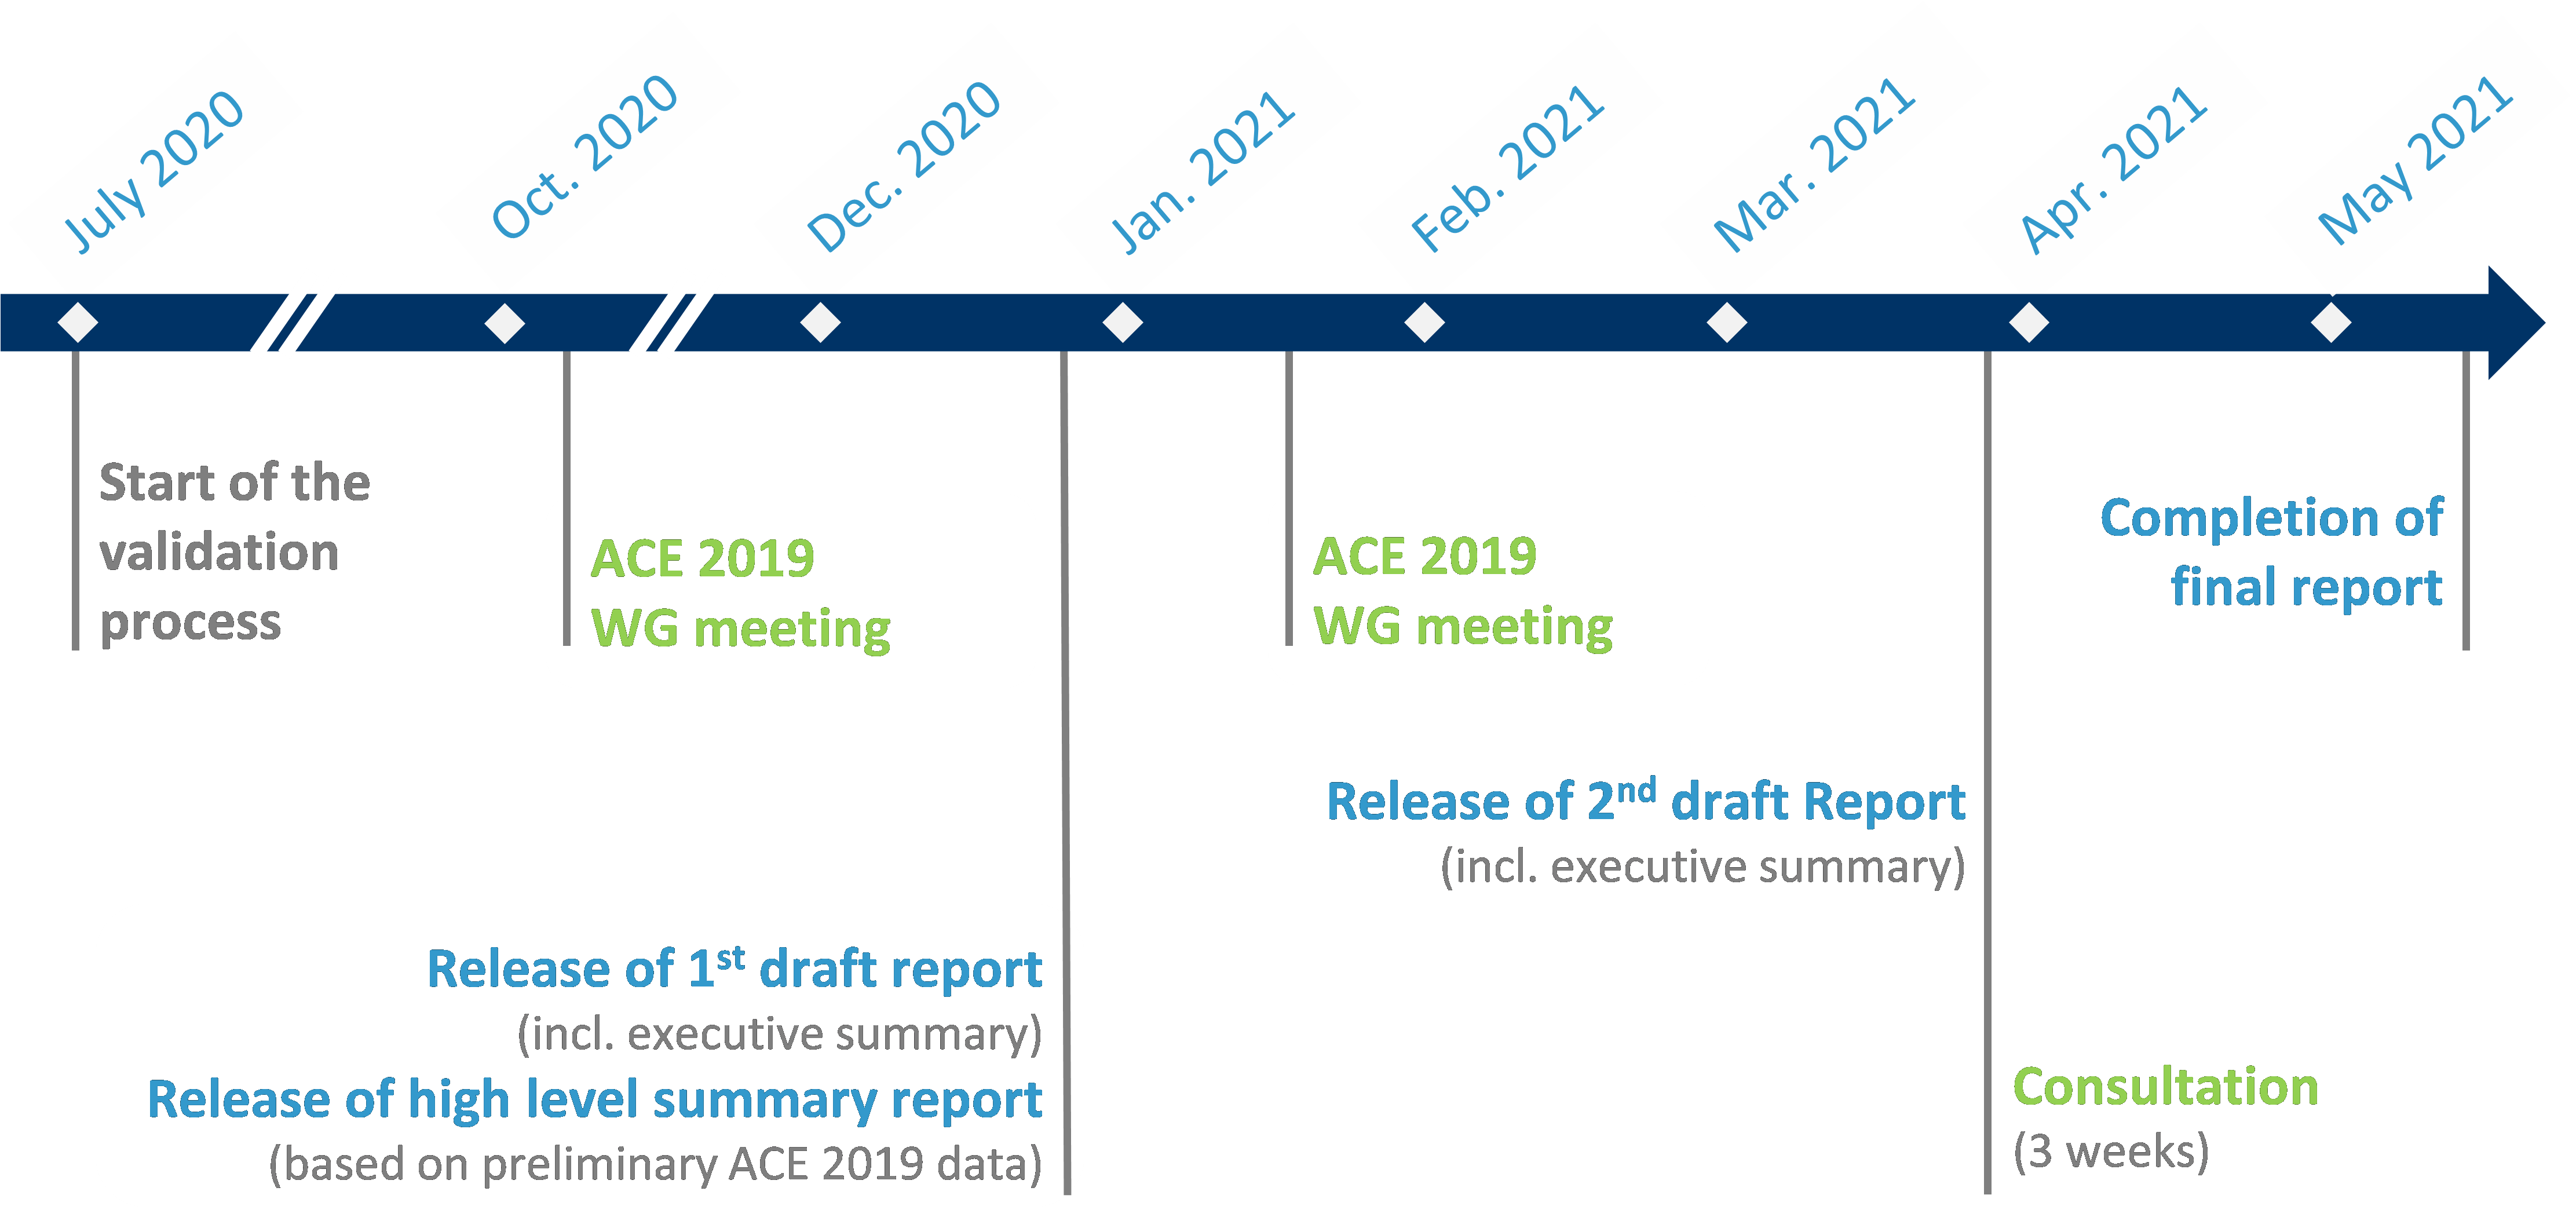
\includegraphics[width=1\linewidth]{figures/Figure 1-1} 

}

\caption{Timeline for the production of the ACE 2019 benchmarking report.}\label{fig:figure1}
\end{figure}

It is important that robust ACE benchmarking analysis is available in a timely manner since several stakeholders, most notably ANSPs' management, regulatory authorities (e.g.~NSAs) and airspace users, have a keen interest in receiving the information in the ACE reports as early as possible.
It should be noted that the data presented in this document are still preliminary and not fully validated. These data reflect the information stored in the ACE database on the 13th November 2020. Figure \ref{fig:figure2} shows the status of the ACE data validation process for the data presented in this document.



\begin{figure}

{\centering 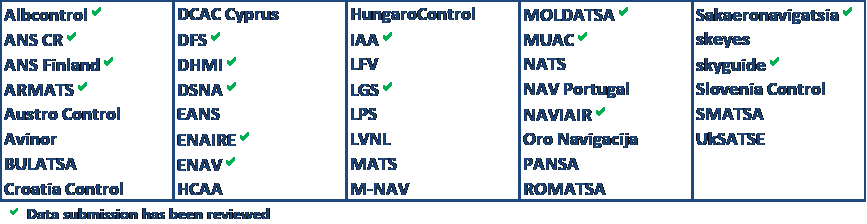
\includegraphics[width=1\linewidth]{figures/Figure 1-2} 

}

\caption{Status of 2019 data validation process.}\label{fig:figure2}
\end{figure}

The data contained in this report is therefore subject to changes before the release of the final ACE 2019 benchmarking report in May 2021.

Figure \ref{fig:figure3} below shows that 23 ANSPs provided their ACE 2019 data submission on time by the 1st July 2019 and that, in total, 26 data submissions were received by the 15th July 2020. Figure \ref{fig:figure2} also indicates that for 11 ANSPs the ACE data submission was received more than one month after the deadline.



\begin{figure}

{\centering 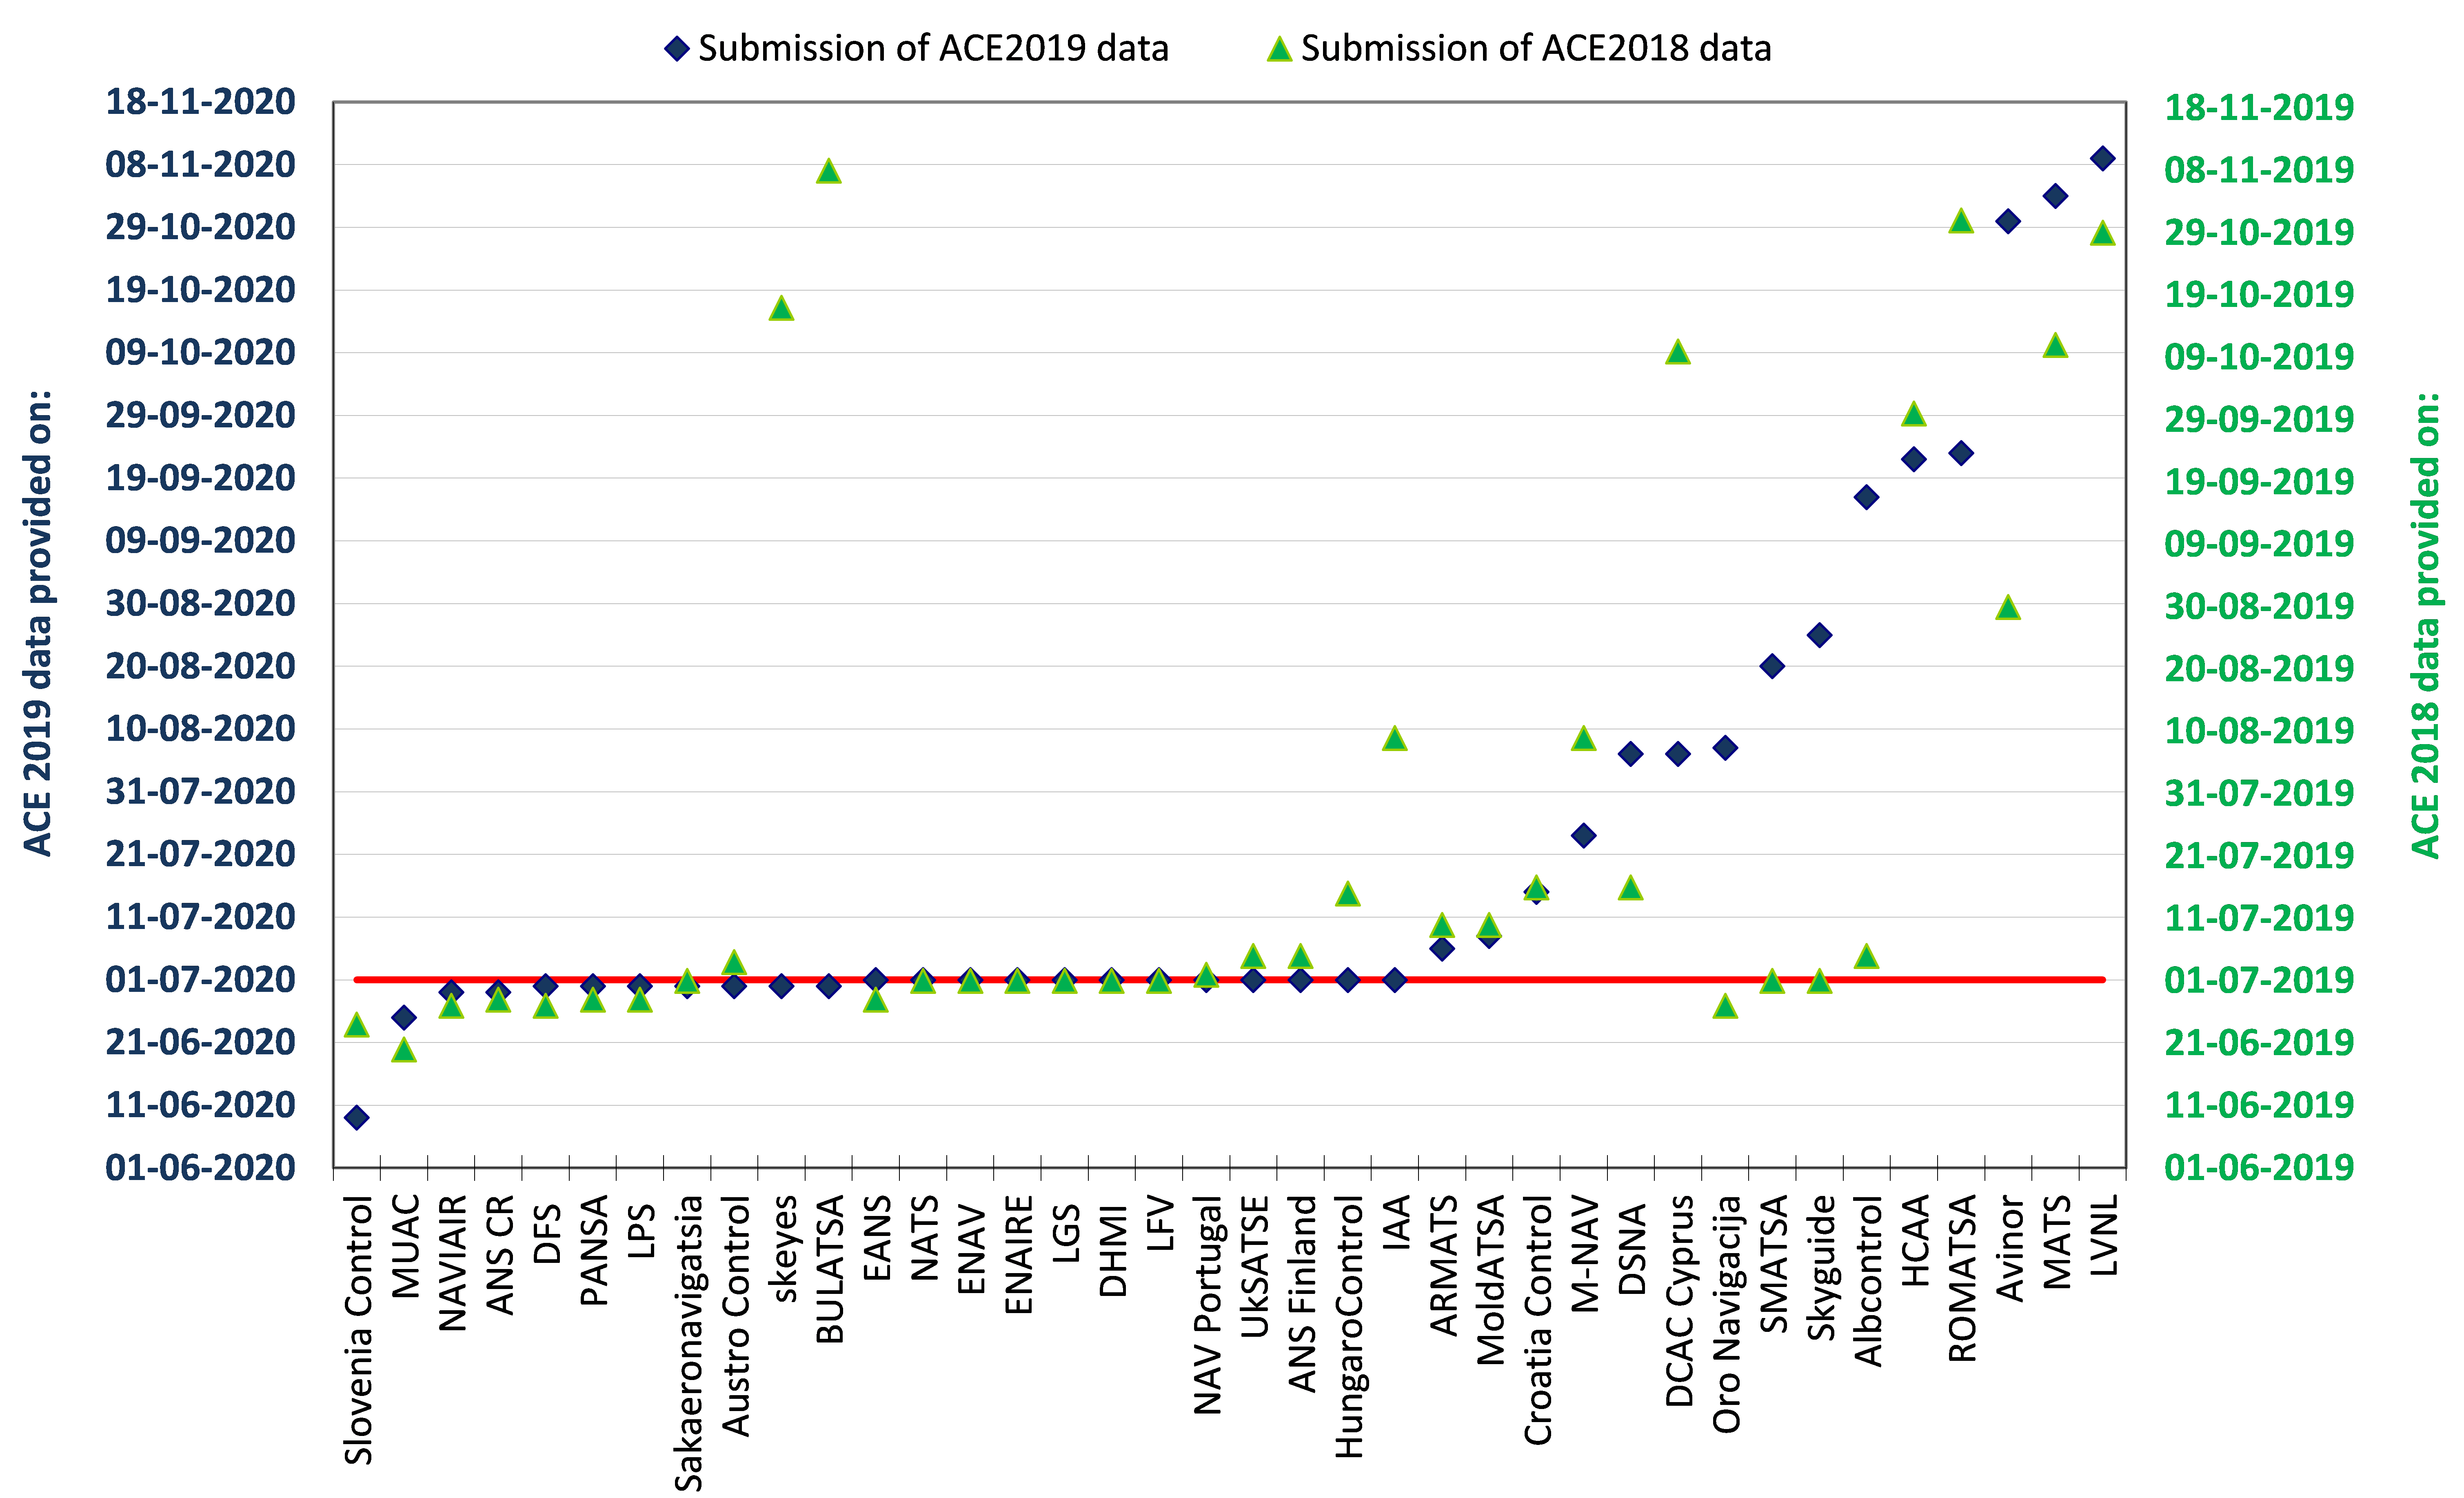
\includegraphics[width=1\linewidth]{figures/Figure 1-3} 

}

\caption{Status of ACE 2019 data submission.}\label{fig:figure3}
\end{figure}

Clearly, the timescale for the production of the ACE benchmarking report is inevitably delayed if data are not submitted on time.
The remainder of this report is organised as follows:

\begin{itemize}
\tightlist
\item
  Section \textbf{\ref{high}}: provides a high-level presentation of 2019 revenues, costs and staff data;
\item
  Section \textbf{\ref{economic}}: presents a preliminary analysis of economic cost-effectiveness at Pan-European and ANSP level;
\item
  Section \textbf{\ref{financial}}: presents a preliminary analysis of financial cost-effectiveness at Pan-European and ANSP level, and underlying components.
\end{itemize}

\hypertarget{high}{%
\chapter{High-level revenues, costs and staff data}\label{high}}

This section provides a preliminary presentation of high-level revenues, costs and staff data provided in ANSPs ACE 2019 data submissions. Total ANS revenues in 2019 amounted to €9 644M. Almost all en-route revenues comes from the collection of en-route charges (95.7\%, see left pie chart). The proportion is lower for terminal revenues (69.0\%, see right pie chart), as additional income may directly come from airport operators (21.2\% e.g.~through a contractual arrangement between the ANSP and the airport operator).



\begin{figure}

{\centering 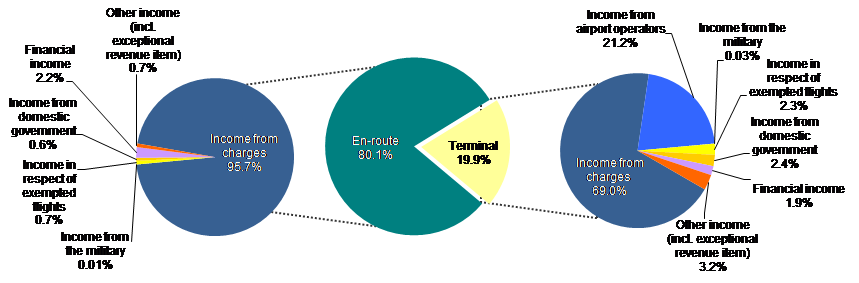
\includegraphics[width=0.5\linewidth]{figures/Figure 2-1-Top} 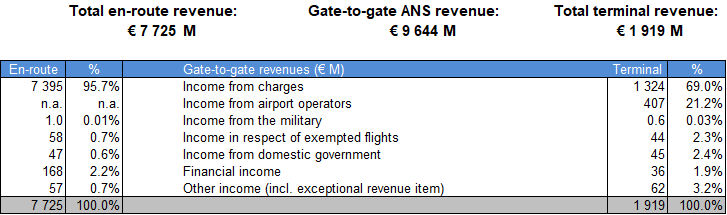
\includegraphics[width=0.5\linewidth]{figures/Figure 2-1-Bottom} 

}

\caption{Breakdown of gate-to-gate ANS revenues, 2019.}\label{fig:figure4}
\end{figure}

From a methodological point of view, the ACE benchmarking analysis focuses on the specific costs of providing gate-to-gate ATM/CNS services which amounted to €8 764M in 2019. Operating costs (including staff costs, non-staff operating costs and exceptional cost items) accounted for some 84\% of total ATM/CNS provision costs, while depreciation costs and the cost of capital represented some 16\%.



\begin{figure}

{\centering 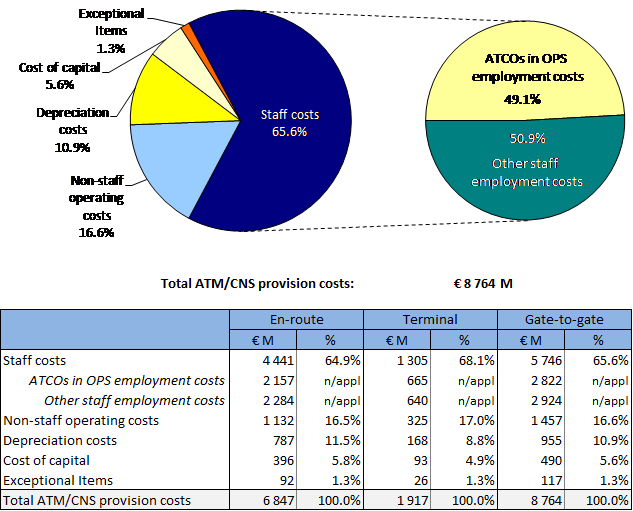
\includegraphics[width=1\linewidth]{figures/Figure 2-2} 

}

\caption{Gate-to-gate ATM/CNS provision costs at Pan-European system level, 2019.}\label{fig:figure5}
\end{figure}

In 2019, the five largest ANSPs (ENAIRE, ENAV, DFS, DSNA and NATS) bore some 54\% of total Pan-European gate-to-gate ATM/CNS provision costs, while the five smallest ANSPs accounted for some 1\% (see bottom left part of Figure \ref{fig:figure6} below). Between 2014 and 2019, ATM/CNS provision costs increased continuously (+1.3\% per annum, on average) at Pan-European system level (see top chart of Figure \ref{fig:figure6}). As shown in the bottom right part of Figure \ref{fig:figure6}, the +2.3\% increase in ATM/CNS costs observed for the Pan-European system in 2019 masks different trends amongst the 37 ANSPs \footnote{Sakaeronavigatsia is excluded from the trend analysis provided in the top chart of Figure \ref{fig:figure6} since no data is available prior to 2015 for this ANSP.}. More details on the changes in ANSPs ATM/CNS provision costs in 2019 will be available in the final ACE 2019 benchmarking report.



\begin{figure}

{\centering 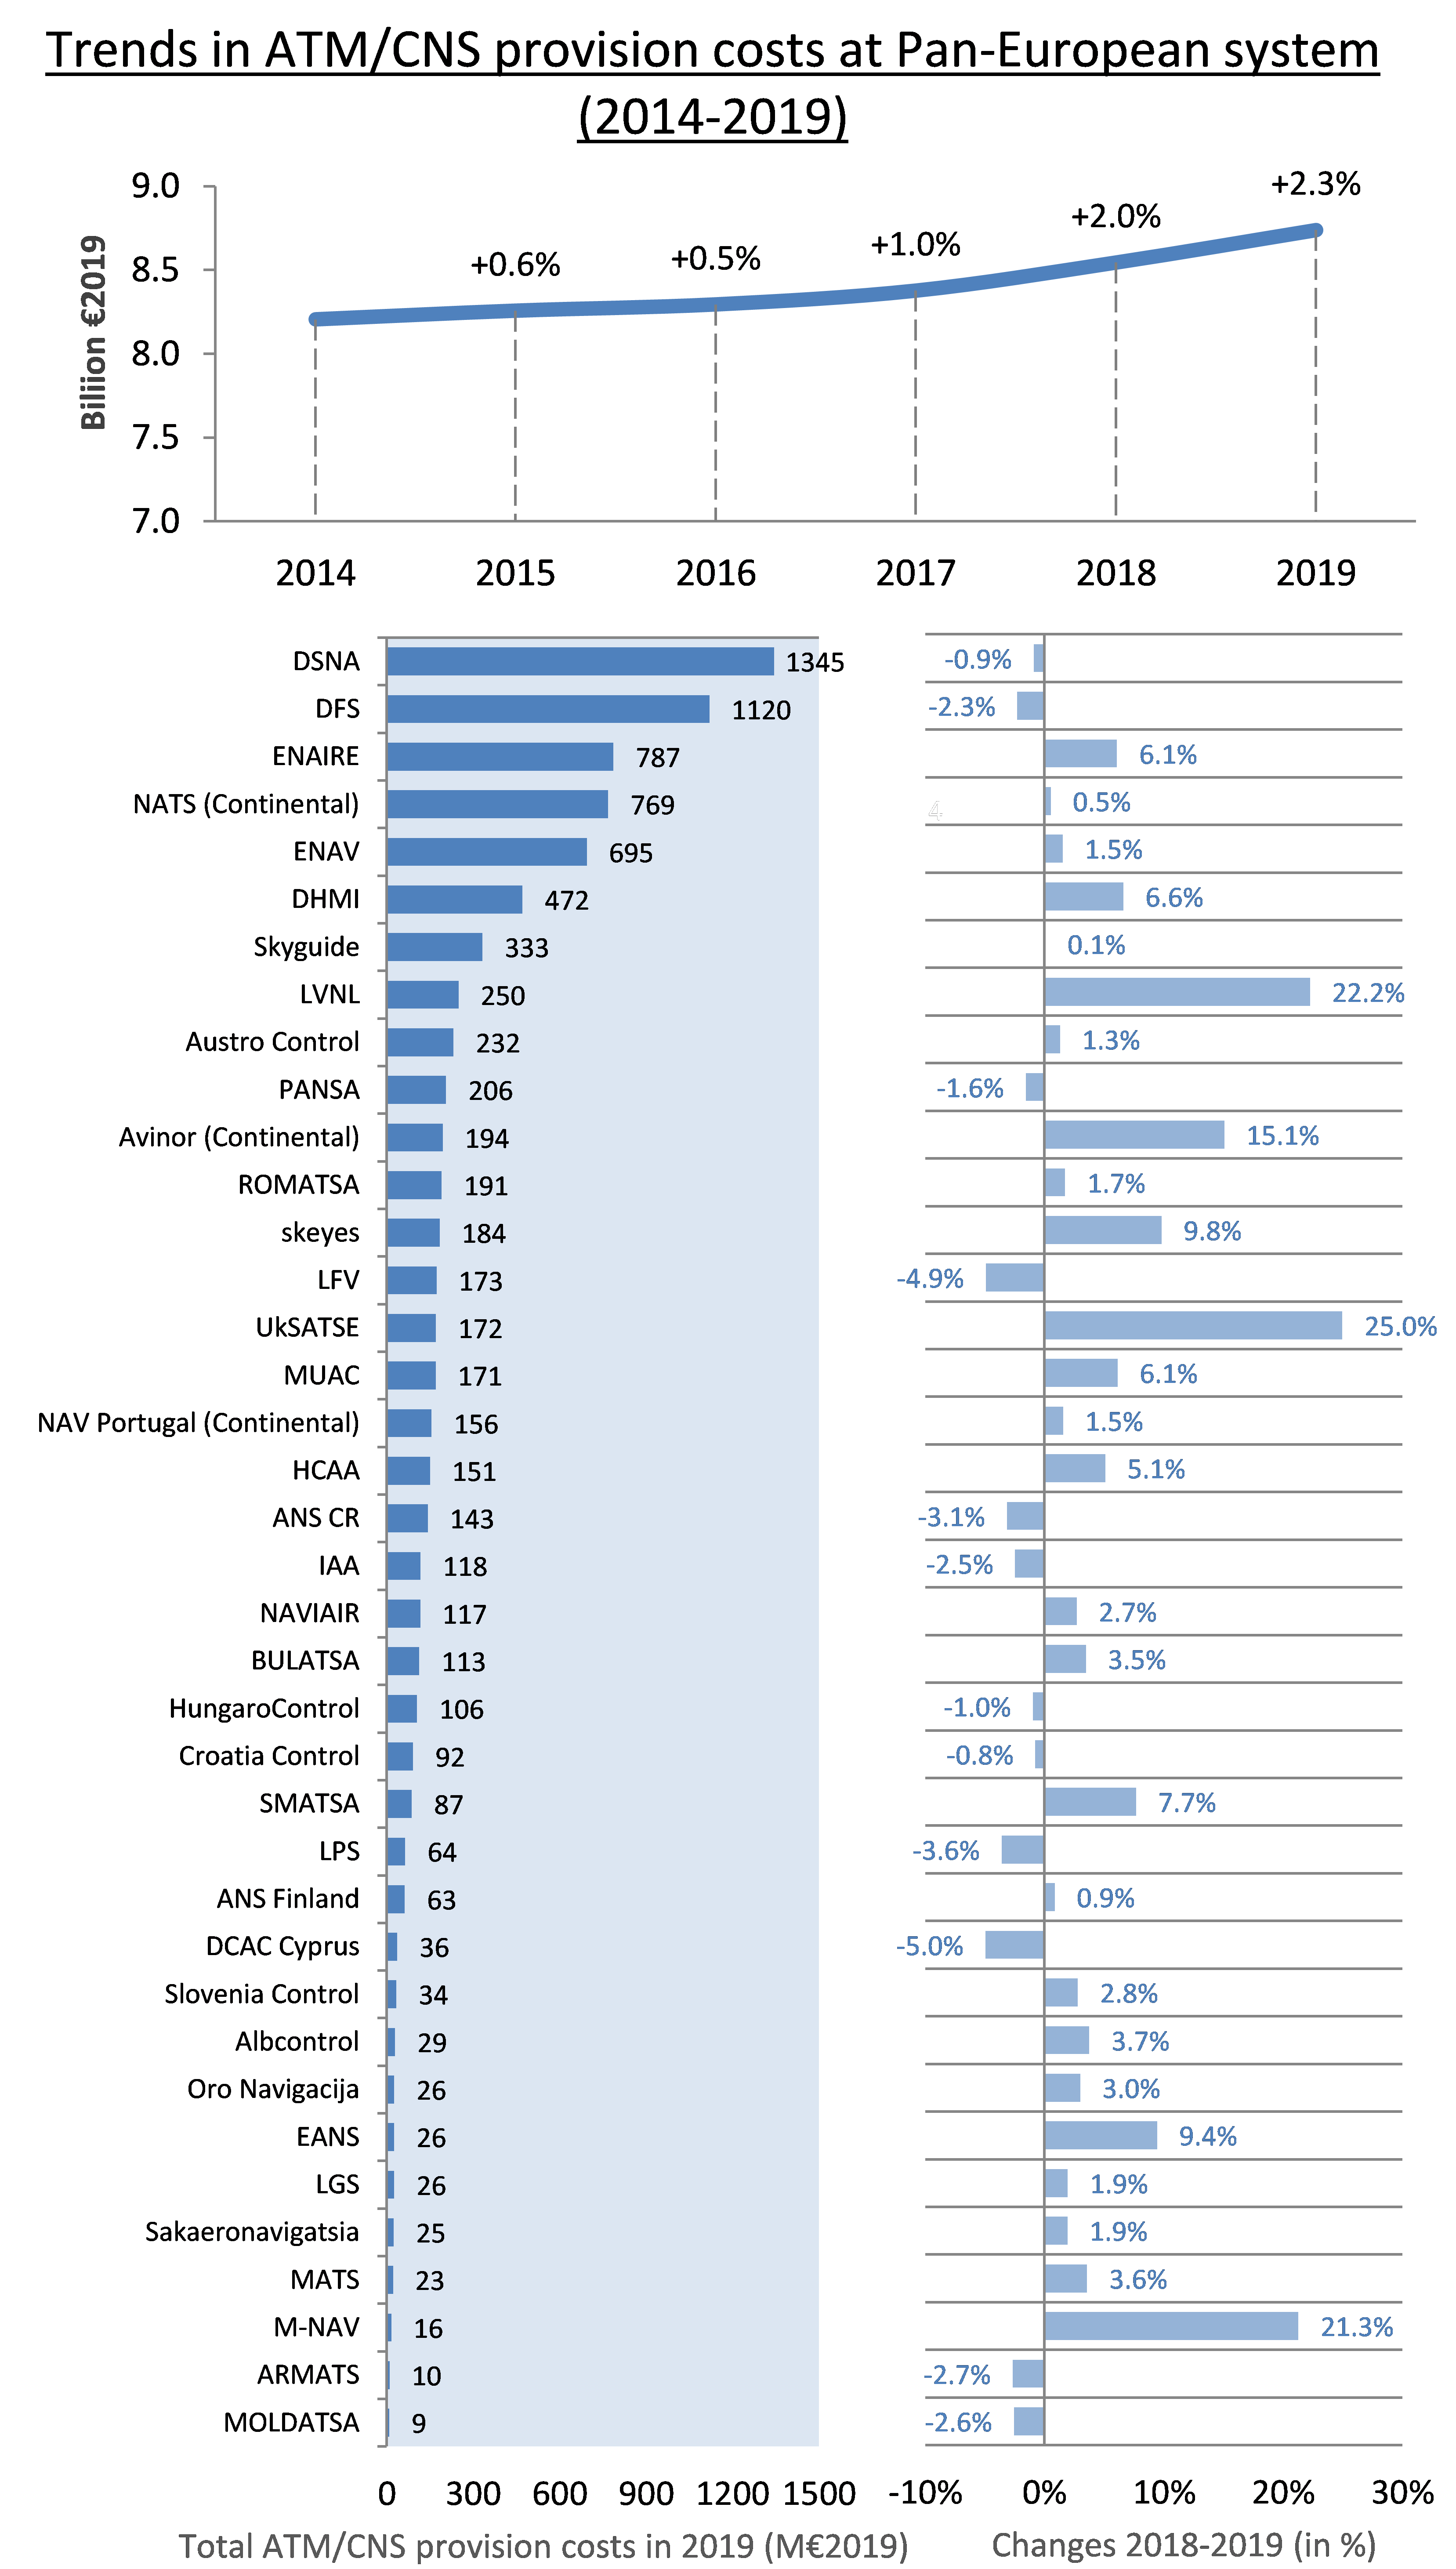
\includegraphics[width=1\linewidth]{figures/Figure 2-3} 

}

\caption{Changes in ATM/CNS provision costs, 2014-2019 (real terms).}\label{fig:figure6}
\end{figure}

The Pan-European ANSPs employed some 56 864 ATM/CNS staff in 2019 (excluding 877 internal MET staff). Some 17 984 staff (32\%) were ATCOs working on operational duty, split between ACCs (56\%) and APP/TWR facilities (44\%). On average, 2.2 additional staff are required for every ATCO in OPS in Europe.



\begin{figure}

{\centering 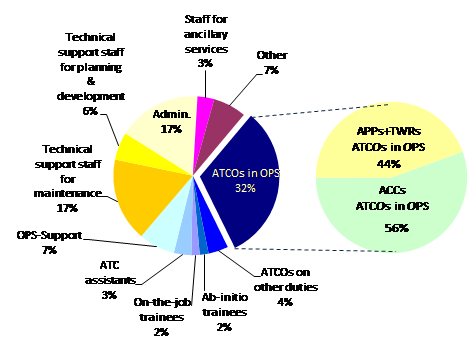
\includegraphics[width=1\linewidth]{figures/Figure 2-4} 

}

\caption{Breakdown of total gate-to-gate ATM/CNS staff at Pan-European system level, 2019.}\label{fig:figure7}
\end{figure}



\begin{cols}

\begin{col}{0.55\textwidth}

\begin{figure}

{\centering 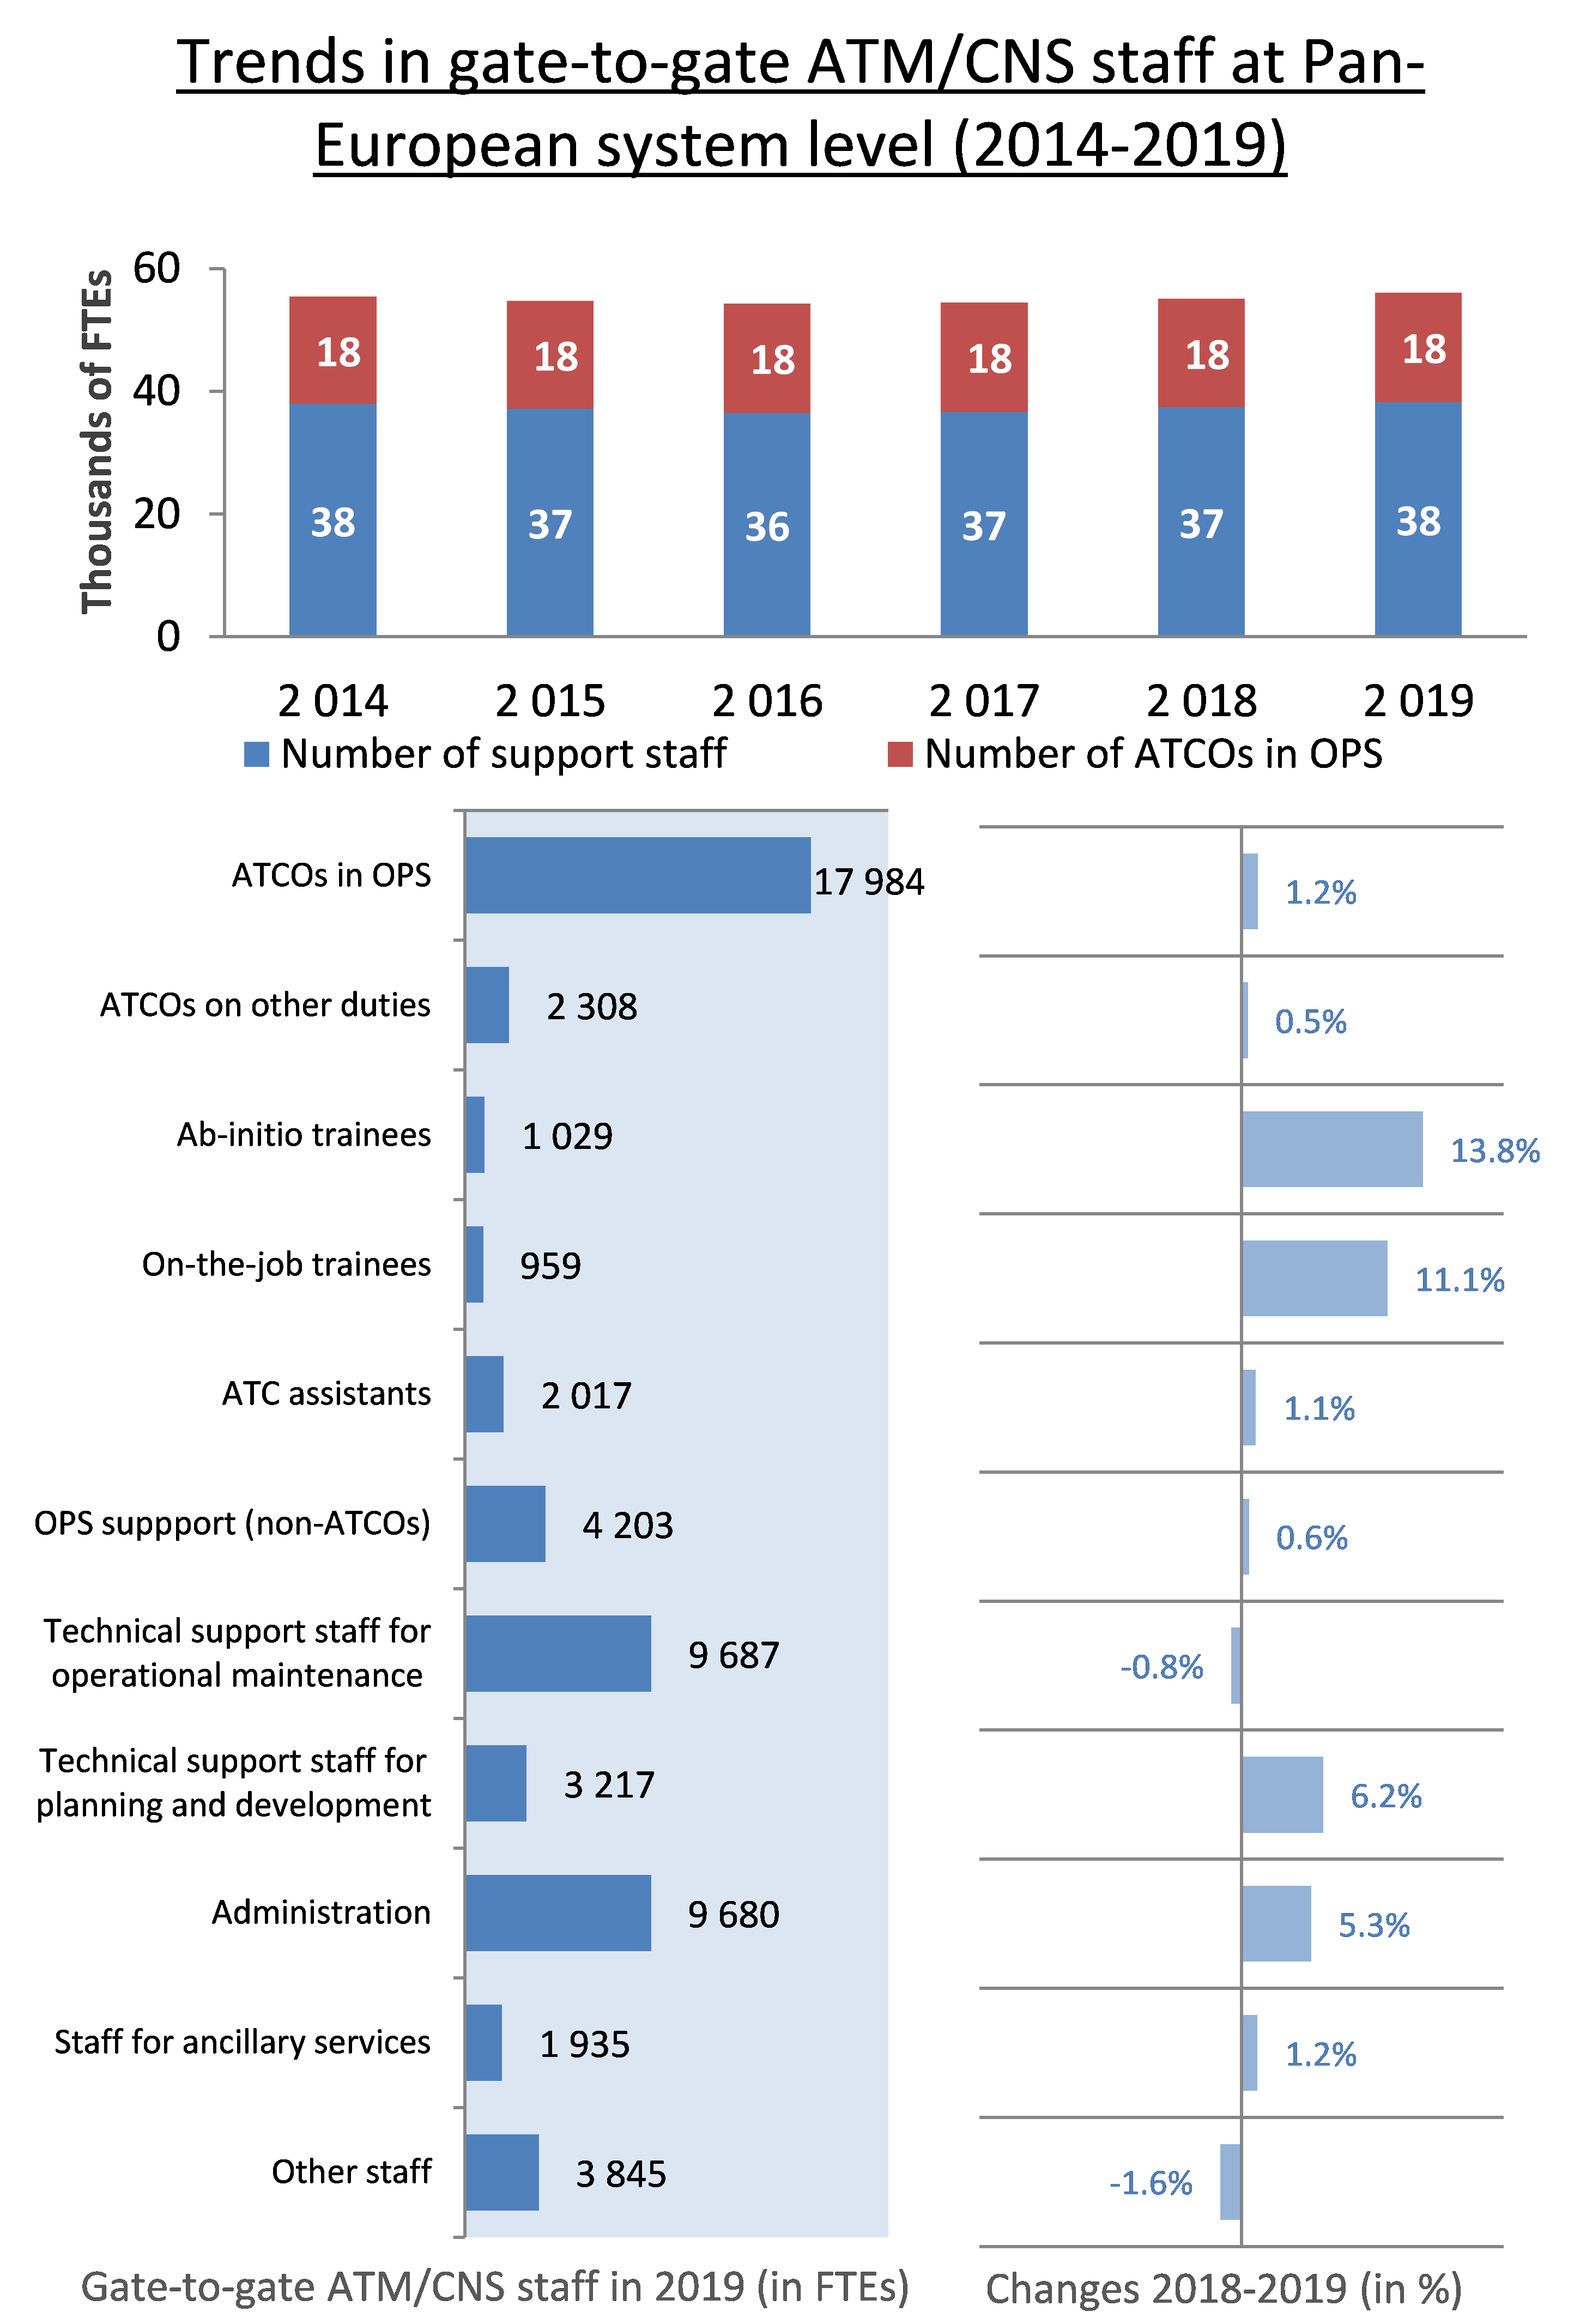
\includegraphics[width=1\linewidth]{figures/Figure 2-5} 

}

\caption{Total gate-to-gate ATM/CNS staff per staff category and changes, 2018-2019\footnote{Sakaeronavigatsia is excluded from the upper part of Figure 2-5 since no data is available prior to 2015 for this ANSP. It is however included in the lower part of the figure as well as in the comments of changes after 2015.}.}\label{fig:figure8}
\end{figure}

\end{col}

\begin{col}{0.05\textwidth}
~

\end{col}

\begin{col}{0.4\textwidth}

Between 2014 and 2019, the number of ATM/CNS staff employed by ANSPs increased by +0.2\% p.a. (some +668 FTEs). After two years of consecutive reductions, the total staff number rose by +0.5\% (+248 FTEs) in 2017, +1.0\% (+554 FTEs) in 2018 and +1.9\% (+1 061 FTEs) in 2019. The higher staff number observed for 2019 mainly reflects increases in the following staff categories:

\begin{itemize}
\tightlist
\item
  Administrative staff (+490 FTEs, or +5.3\%);
\item
  ATCOs in OPS (+220 FTEs, or +1.2\%);
\item
  Technical support for planning and development (+189 FTEs, or +6.2\%);
\item
  Ab-initio trainees (+125 FTEs, or +13.8\%);
\item
  On-the-job trainees (+96 FTEs, or +11.1\%). On the other hand, relatively small decreases are observed for support staff for operational maintenance (-77 FTEs, or -0.8\%) and other staff (-63 FTEs, or - 1.6\%).
\end{itemize}

\end{col}

\end{cols}

\hypertarget{economic}{%
\chapter{Economic cost-effectiveness}\label{economic}}

This section provides a preliminary analysis of economic cost-effectiveness at Pan-European and ANSP level.

\hypertarget{pan-european-system-level}{%
\section{Pan-European system level}\label{pan-european-system-level}}

The PRC introduced in its ACE benchmarking reports the concept of economic cost-effectiveness. This indicator is defined as gate-to-gate ATM/CNS provision costs plus the costs of ground ATFM delays for both en‐route and airport, all expressed per composite flight-hour. This economic performance indicator is meant to capture trade‐offs between ATC capacity and costs\footnote{See Annex 2 of the ACE 2018 benchmarking report for more information on the methodology used to compute composite flight-hours and economic costs.}. Figure \ref{fig:figure9} analyses the changes in economic cost-effectiveness between 2014 and 2019 at Pan-European system level. The left-hand side of Figure \ref{fig:figure9} shows the changes in unit economic costs, while the right-hand side provides complementary information on the year-on-year changes in ATM/CNS provision costs, composite flight-hours and unit costs of ATFM delays.



\begin{figure}

{\centering 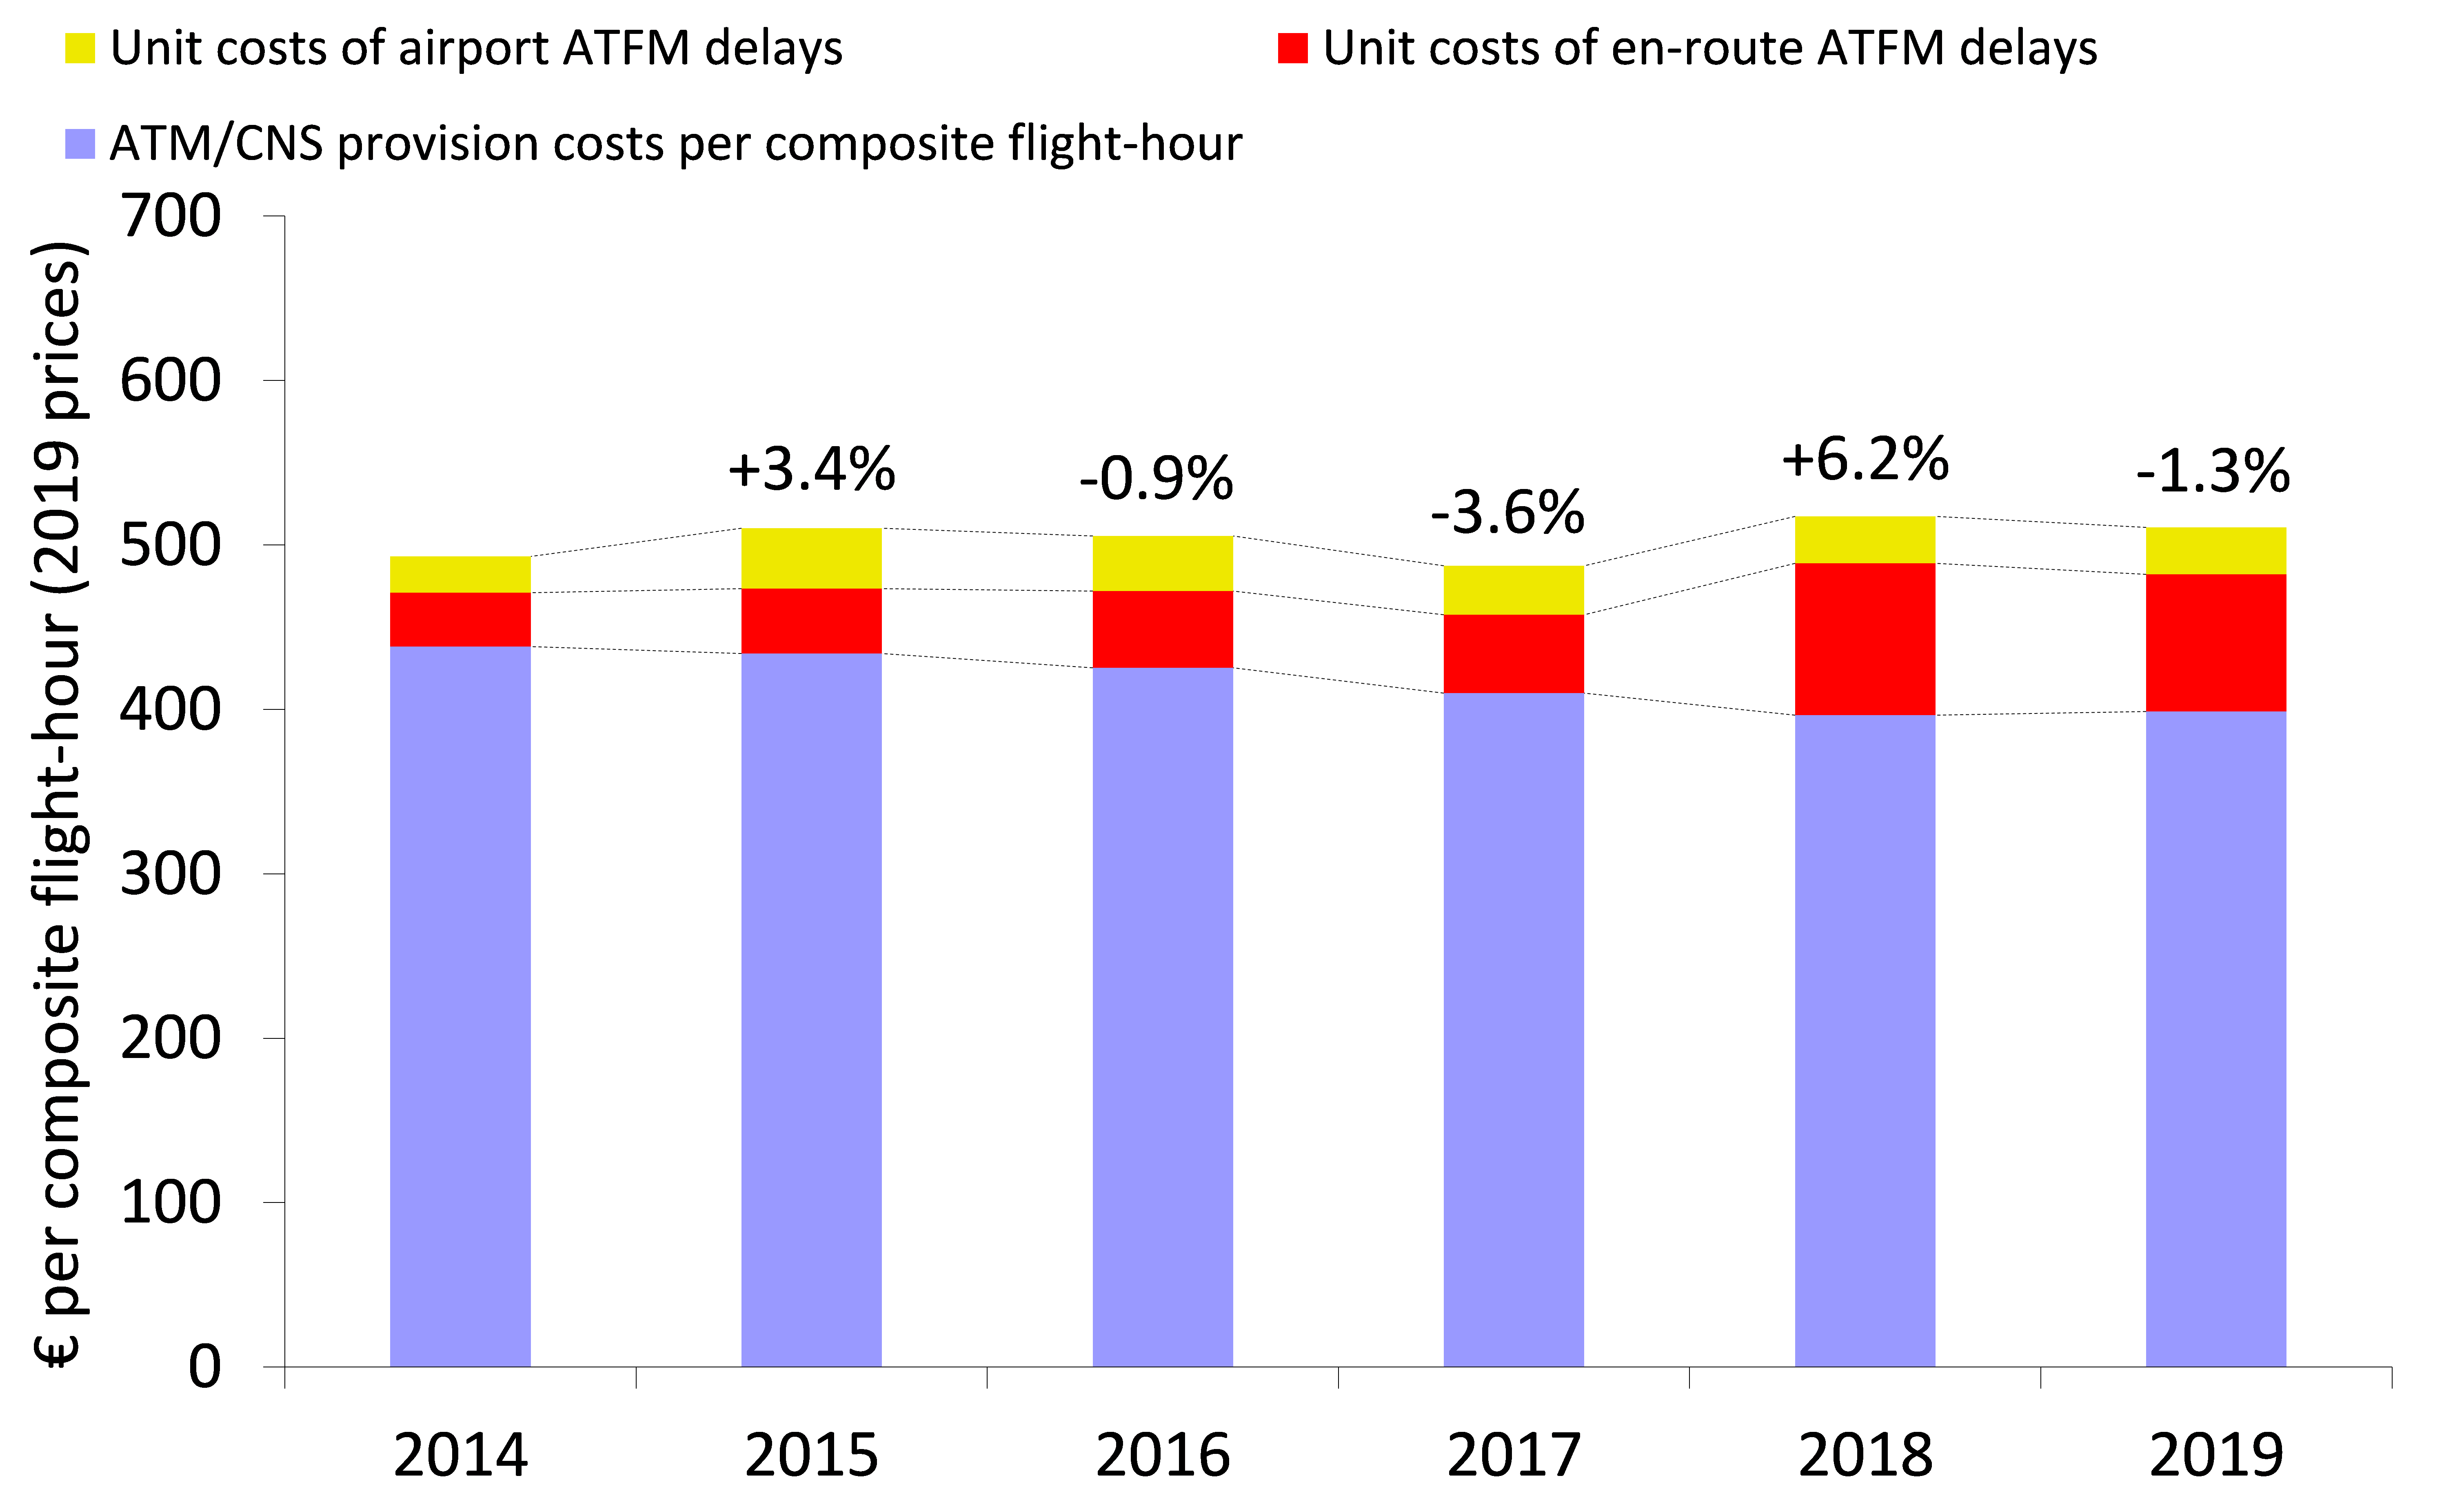
\includegraphics[width=0.5\linewidth]{figures/Figure 3-1-Left} 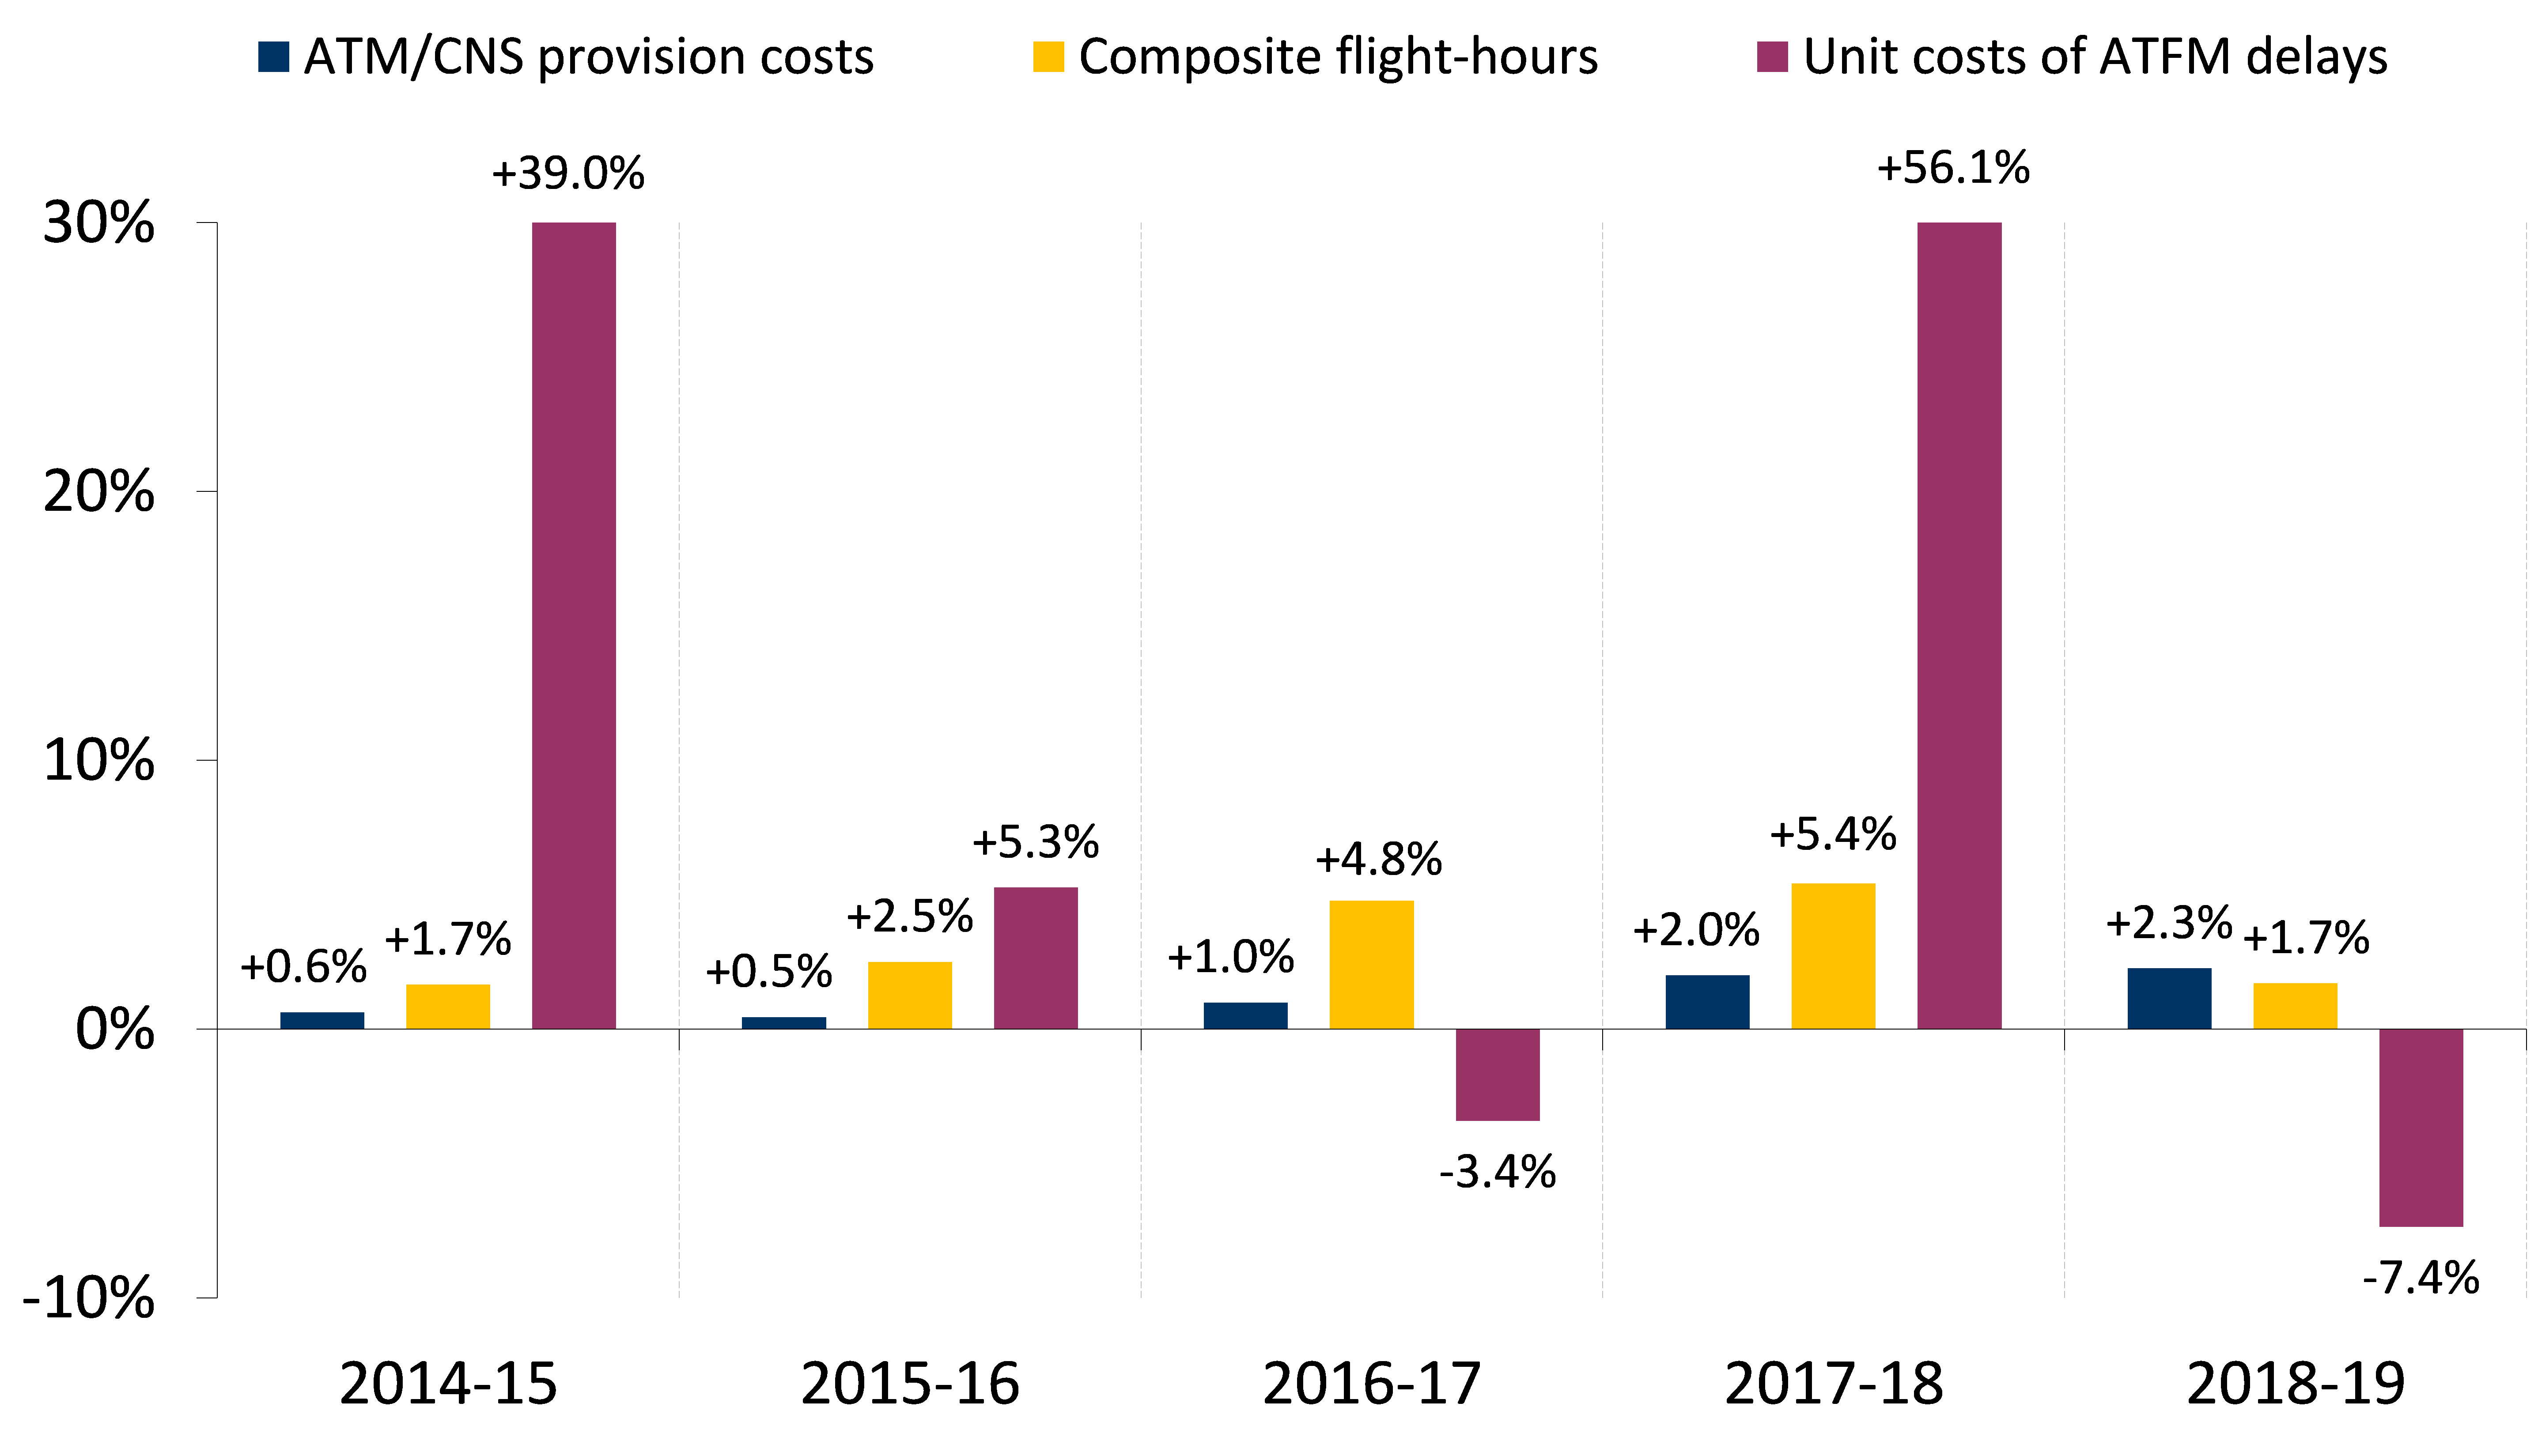
\includegraphics[width=0.5\linewidth]{figures/Figure 3-1-Right} 

}

\caption{Trend of unit economic costs at Pan-European system level, 2014-2019 (real terms)\footnote{Sakaeronavigatsia is excluded from the trend analysis provided in this section since no data is available prior to 2015 for this ANSP.}.}\label{fig:figure9}
\end{figure}

Between 2014 and 2019, economic costs per composite flight-hour increased by +0.7\% p.a. in real terms. Over this period, ATM/CNS provision costs increased continuously (+1.3\% p.a.) in the context of a significant growth in composite flight-hours (+3.2\% p.a.). At the same time, the unit costs of ATFM delays rose by +15.4\% p.a., on average, over the period. In 2019, composite flight-hours rose slower (+1.7\%) than ATM/CNS provision costs (+2.3\%). As a result, unit ATM/CNS provision costs increased by +0.6\%. However, this increase was more than compensated by a substantial reduction in the unit costs of ATFM delays in 2019 (-7.4\%) and therefore unit economic costs decreased by -1.3\% compared to 2018.

\hypertarget{ansp-level}{%
\section{ANSP level}\label{ansp-level}}

The economic cost-effectiveness indicator at Pan-European level amounts to €511 per composite flight-hour, and, on average, the unit costs of ATFM delays represent some 22\% of the unit economic costs.



\begin{figure}

{\centering 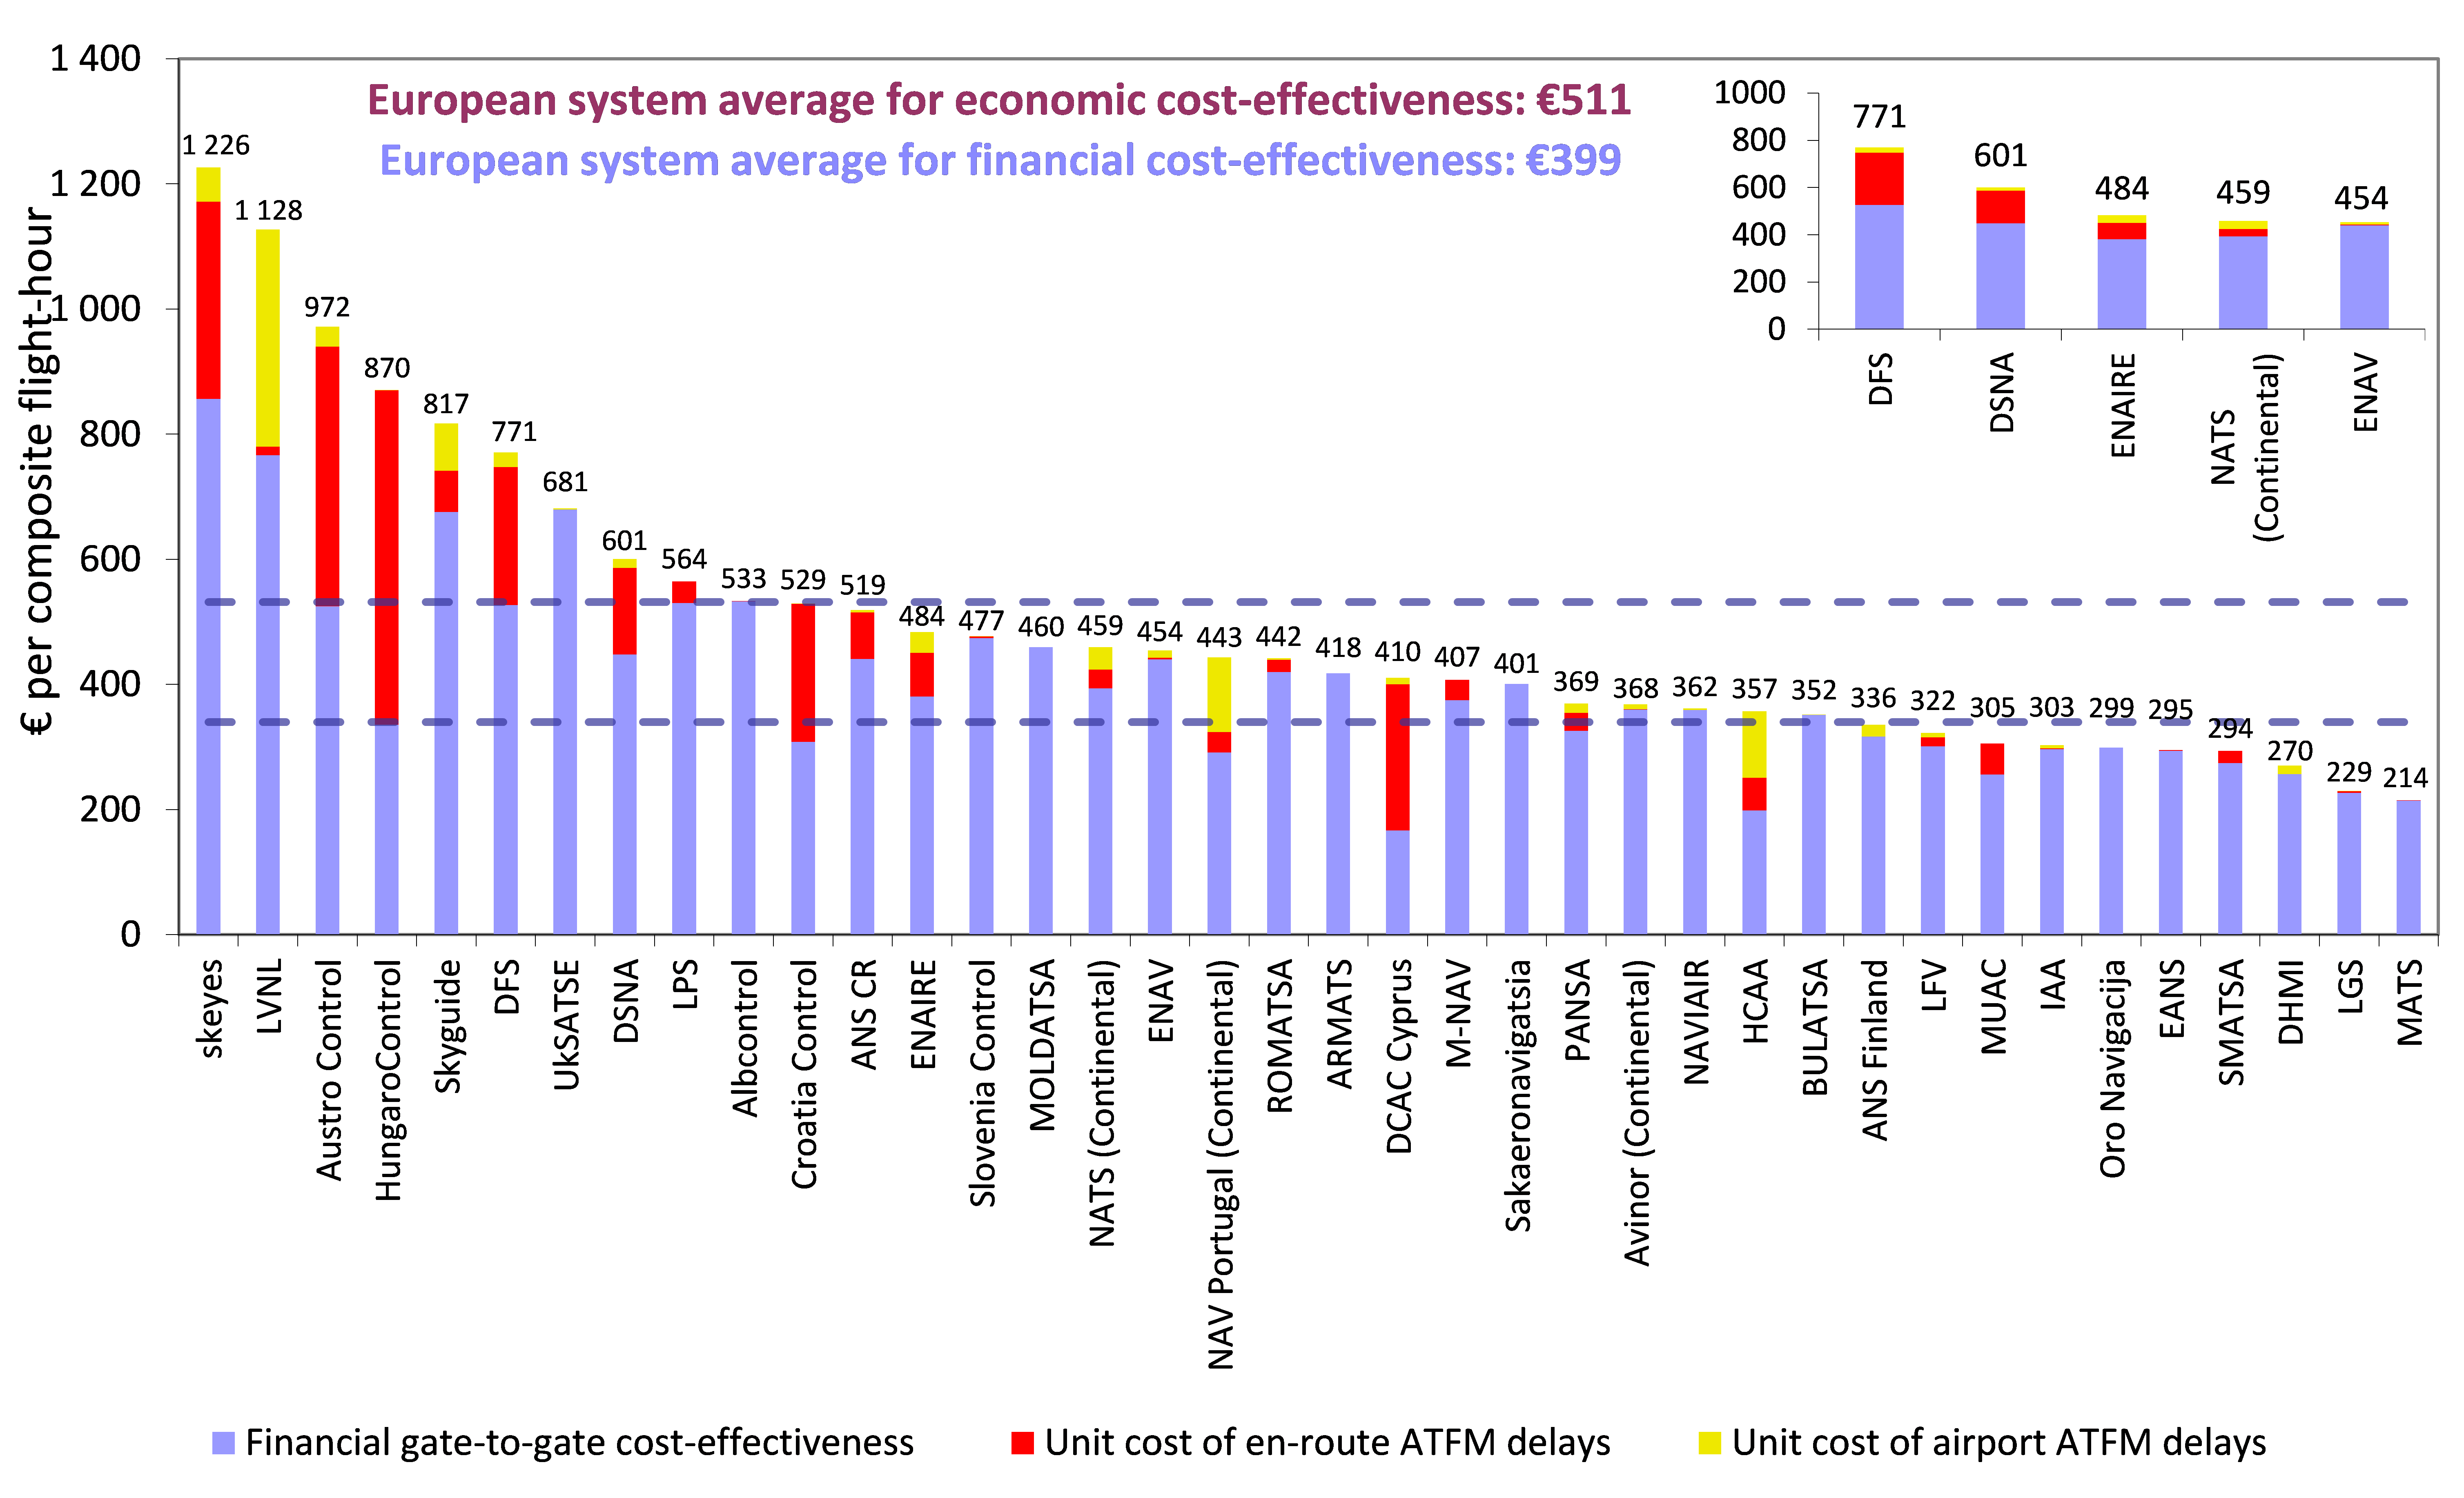
\includegraphics[width=1\linewidth]{figures/Figure 3-2} 

}

\caption{Economic gate-to-gate cost-effectiveness\footnote{For the purposes of the ACE benchmarking analysis, costs relating to ATM/CNS infrastructure shared with the military authority (€20.0M) are included in ENAIRE 2019 ATM/CNS provision costs. These costs, which are charged to civil airspace users, are not passing through ENAIRE Accounts from 2014 onwards but are borne by the Spanish Air Force (Ministry of Defence) as well as corresponding revenues. Without these costs, ENAIRE unit economic costs would be slightly lower and would amount to €474.}, 2019.}\label{fig:figure10}
\end{figure}

More details on the changes in ATFM delays\footnote{The ATFM delays analysed in this ACE benchmarking report do not comprise changes due to the Post Operations Performance Adjustment Process. This process allows operational stakeholders to notify national and European authorities of issues that relate to ATFM delay measurement, classification and assignment. It is a mean of enhancing operational ATFM delay data used in the performance scheme (Commission Implementing Regulation (EU) No 390/2013). The minutes of ATFM delays resulting from this process would lead to different unit economic costs figures for some ANSPs. Detailed information on this process is available on the Network Manager website at the following link: \url{https://www.eurocontrol.int/service/post-operations-performance-adjustment}.} for individual ANSPs will be provided in the ACE 2019 benchmarking report.

\hypertarget{financial}{%
\chapter{Financial cost-effectiveness}\label{financial}}

This section provides a preliminary analysis of financial cost-effectiveness at Pan-European and ANSP level.

\hypertarget{pan-european-system-level}{%
\section{Pan-European system level}\label{pan-european-system-level}}

In 2019, ATM/CNS provision costs (+2.3\%) increased faster than composite flight-hours (+1.7\%) and as a result unit ATM/CNS provision costs rose by +0.6\%.



\begin{figure}

{\centering 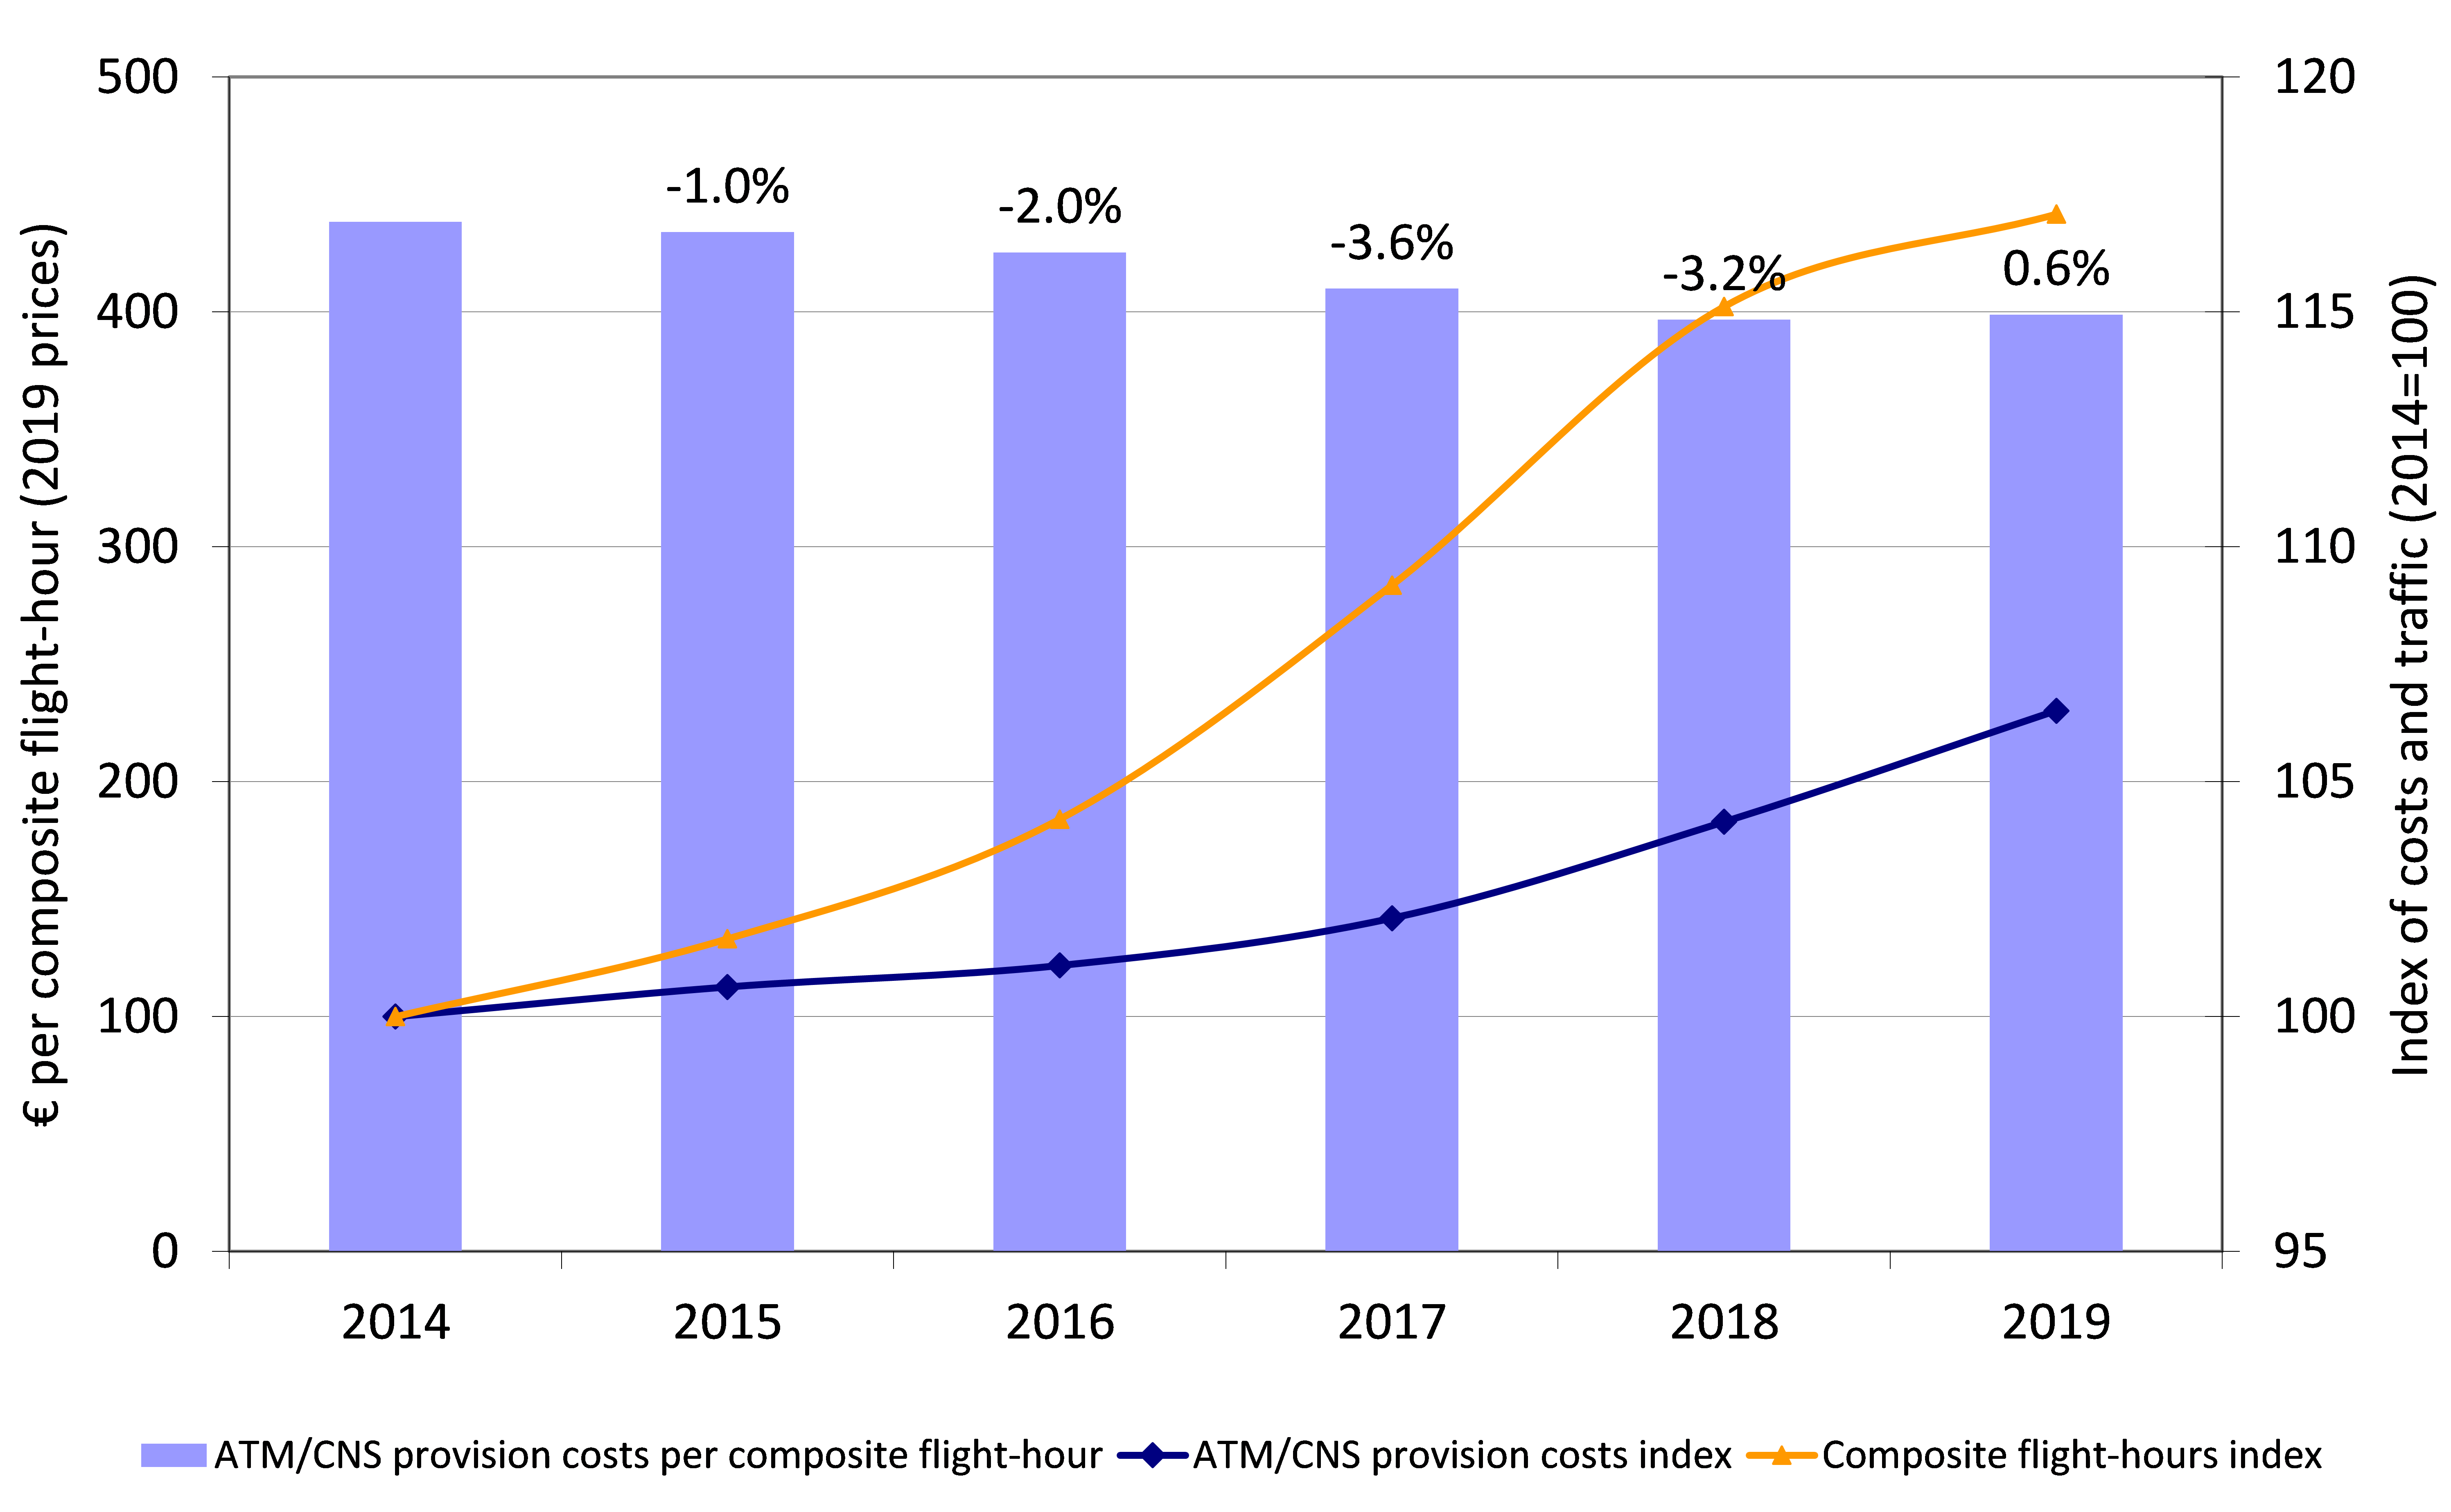
\includegraphics[width=1\linewidth]{figures/Figure 4-1} 

}

\caption{Changes in unit ATM/CNS provision costs, 2014-2019 (real terms).}\label{fig:figure11}
\end{figure}

Figure \ref{fig:figure12} shows the analytical framework which is used in the ACE analysis to break down the financial cost-effectiveness indicator into basic economic drivers. These key drivers include:

\begin{itemize}
\tightlist
\item
  ATCO-hour productivity (0.93 composite flight-hours per ATCO-hour);
\item
  ATCO employment costs per ATCO-hour (€120); and,
\item
  support costs per unit output (€270).
\end{itemize}



\begin{figure}

{\centering 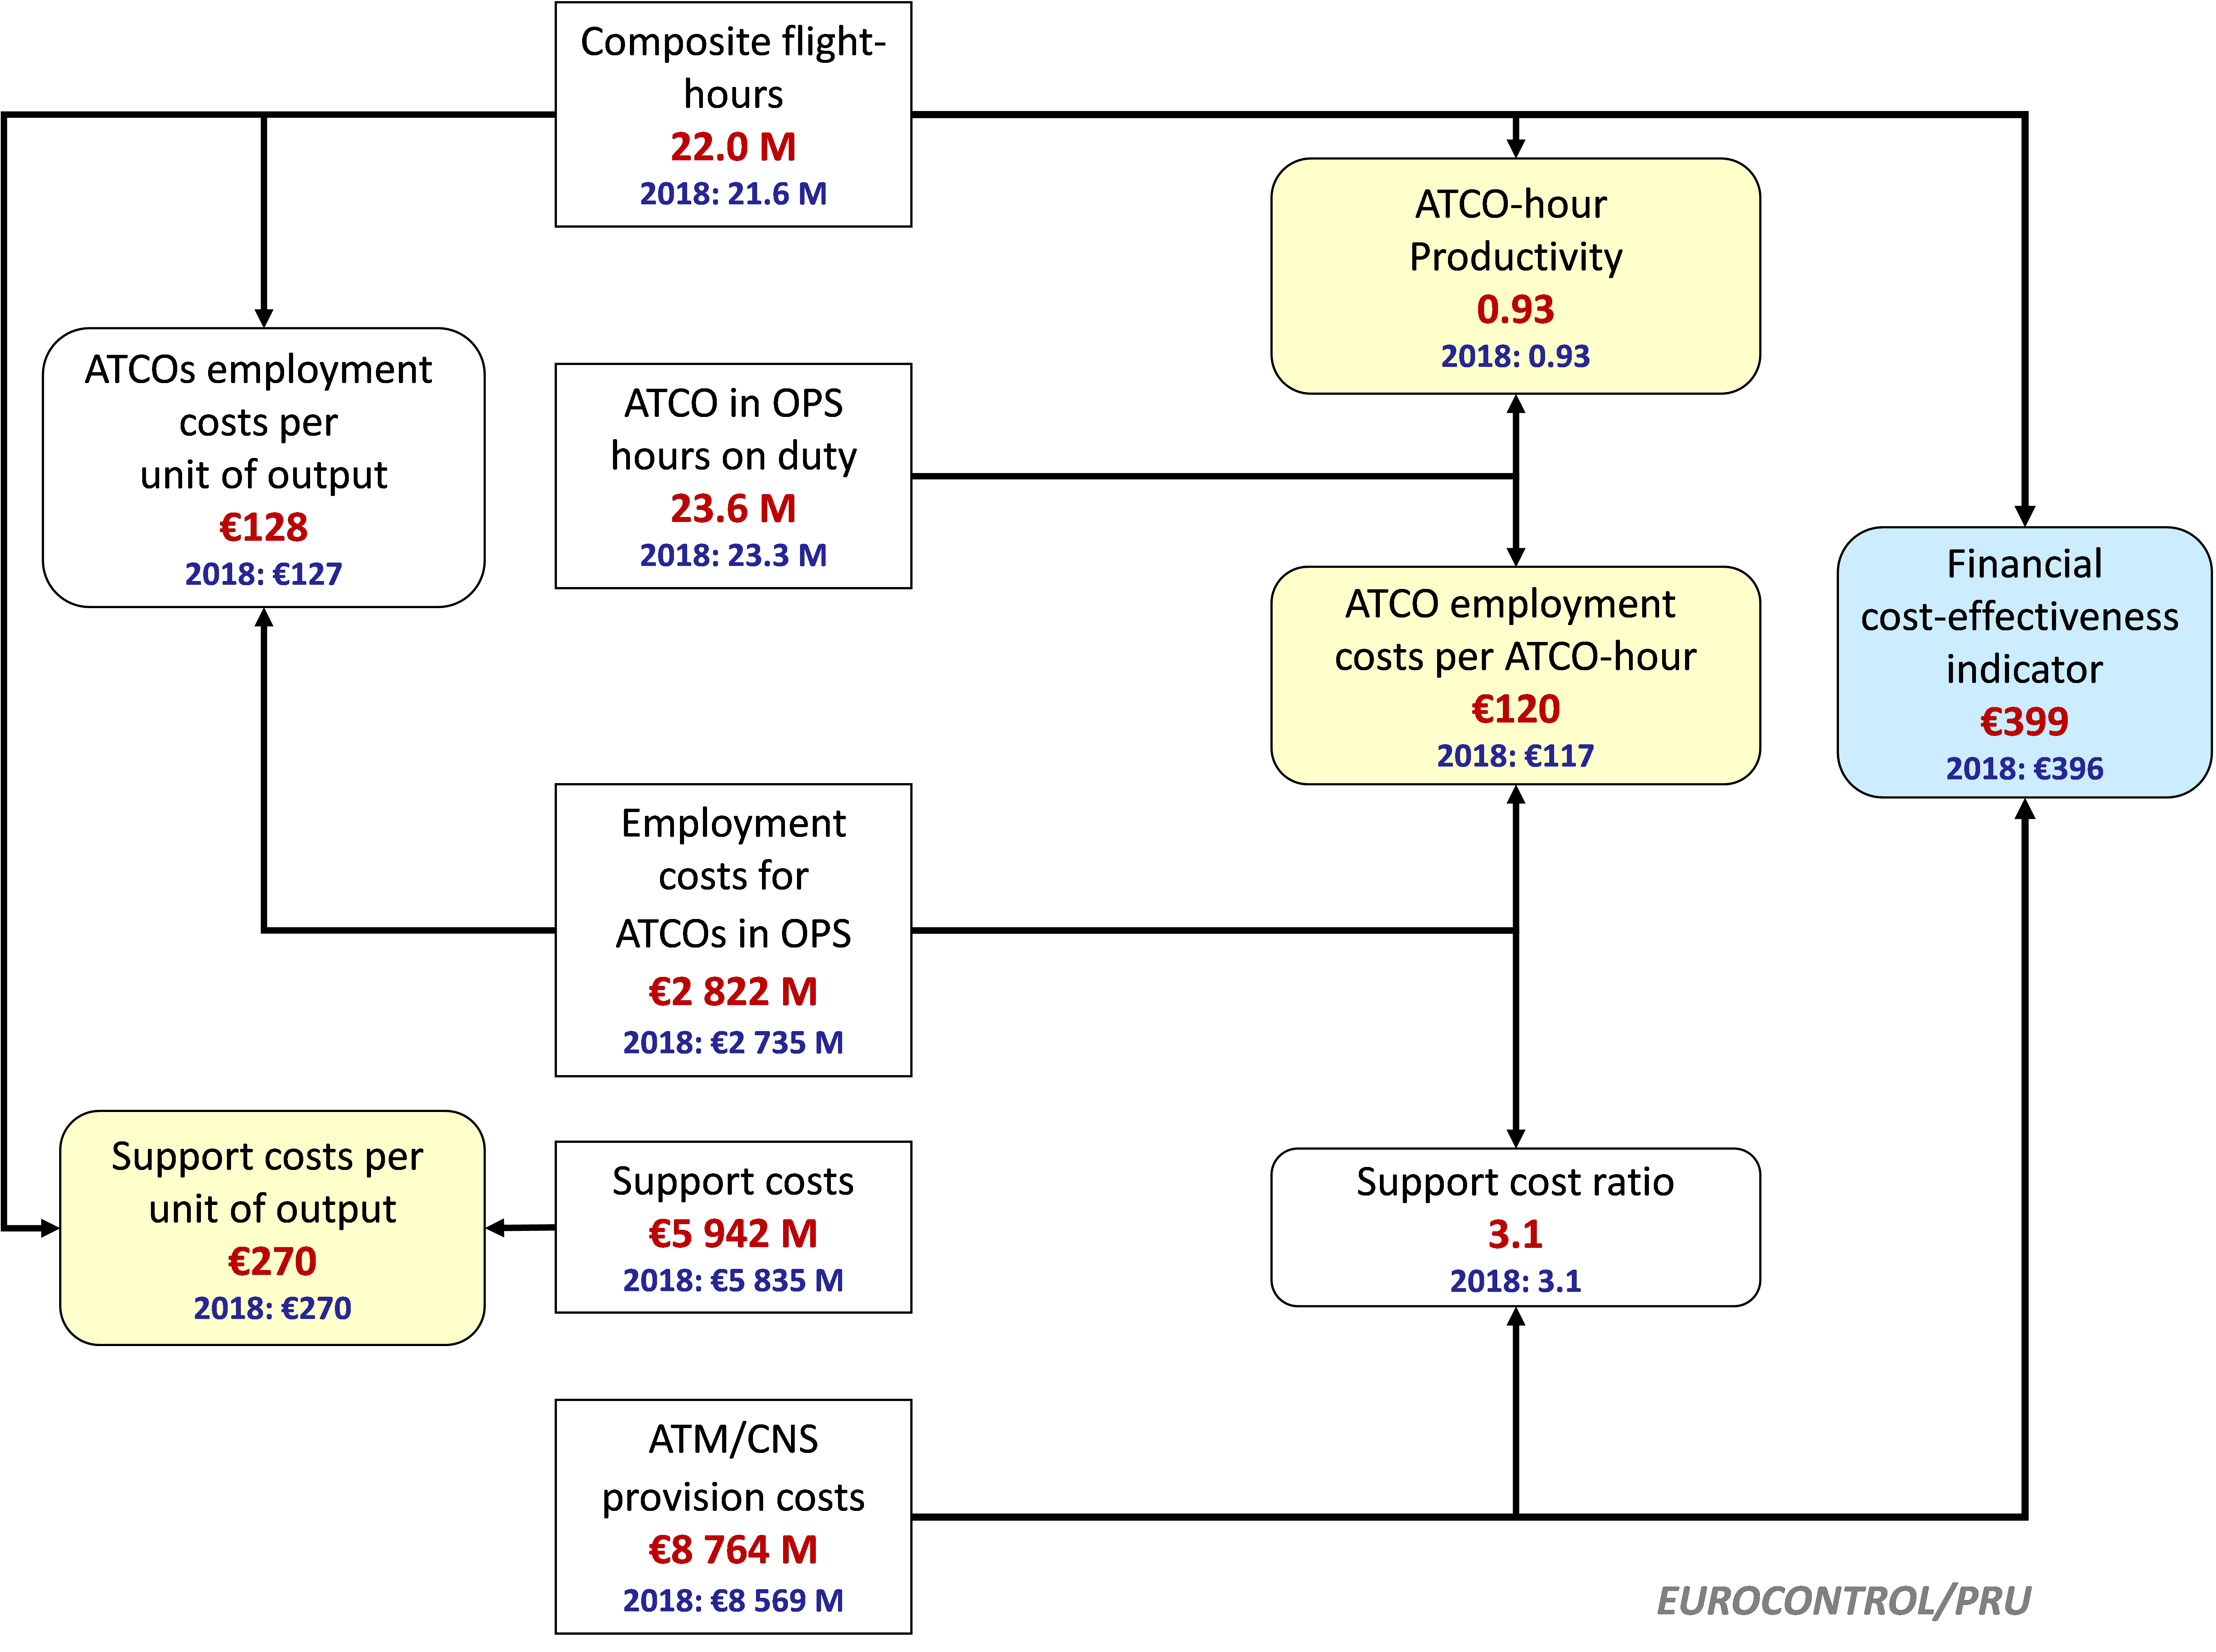
\includegraphics[width=1\linewidth]{figures/Figure 4-2} 

}

\caption{ACE performance framework, 2019 (real terms).}\label{fig:figure12}
\end{figure}

Figure \ref{fig:figure13} below shows that in 2019, ATCO employment costs per ATCO-hour rose faster (+1.9\%) than ATCO-hour productivity (+0.4\%). As a result, ATCO employment costs per composite flight-hour increased (+1.5\%). In the meantime, unit support costs remained almost stable (+0.2\%) since composite flight-hours (+1.7\%) and support costs (+1.8\%) rose at a similar pace. As a result, in 2019 unit ATM/CNS provision costs increased by +0.6\% at Pan-European system level.



\begin{figure}

{\centering 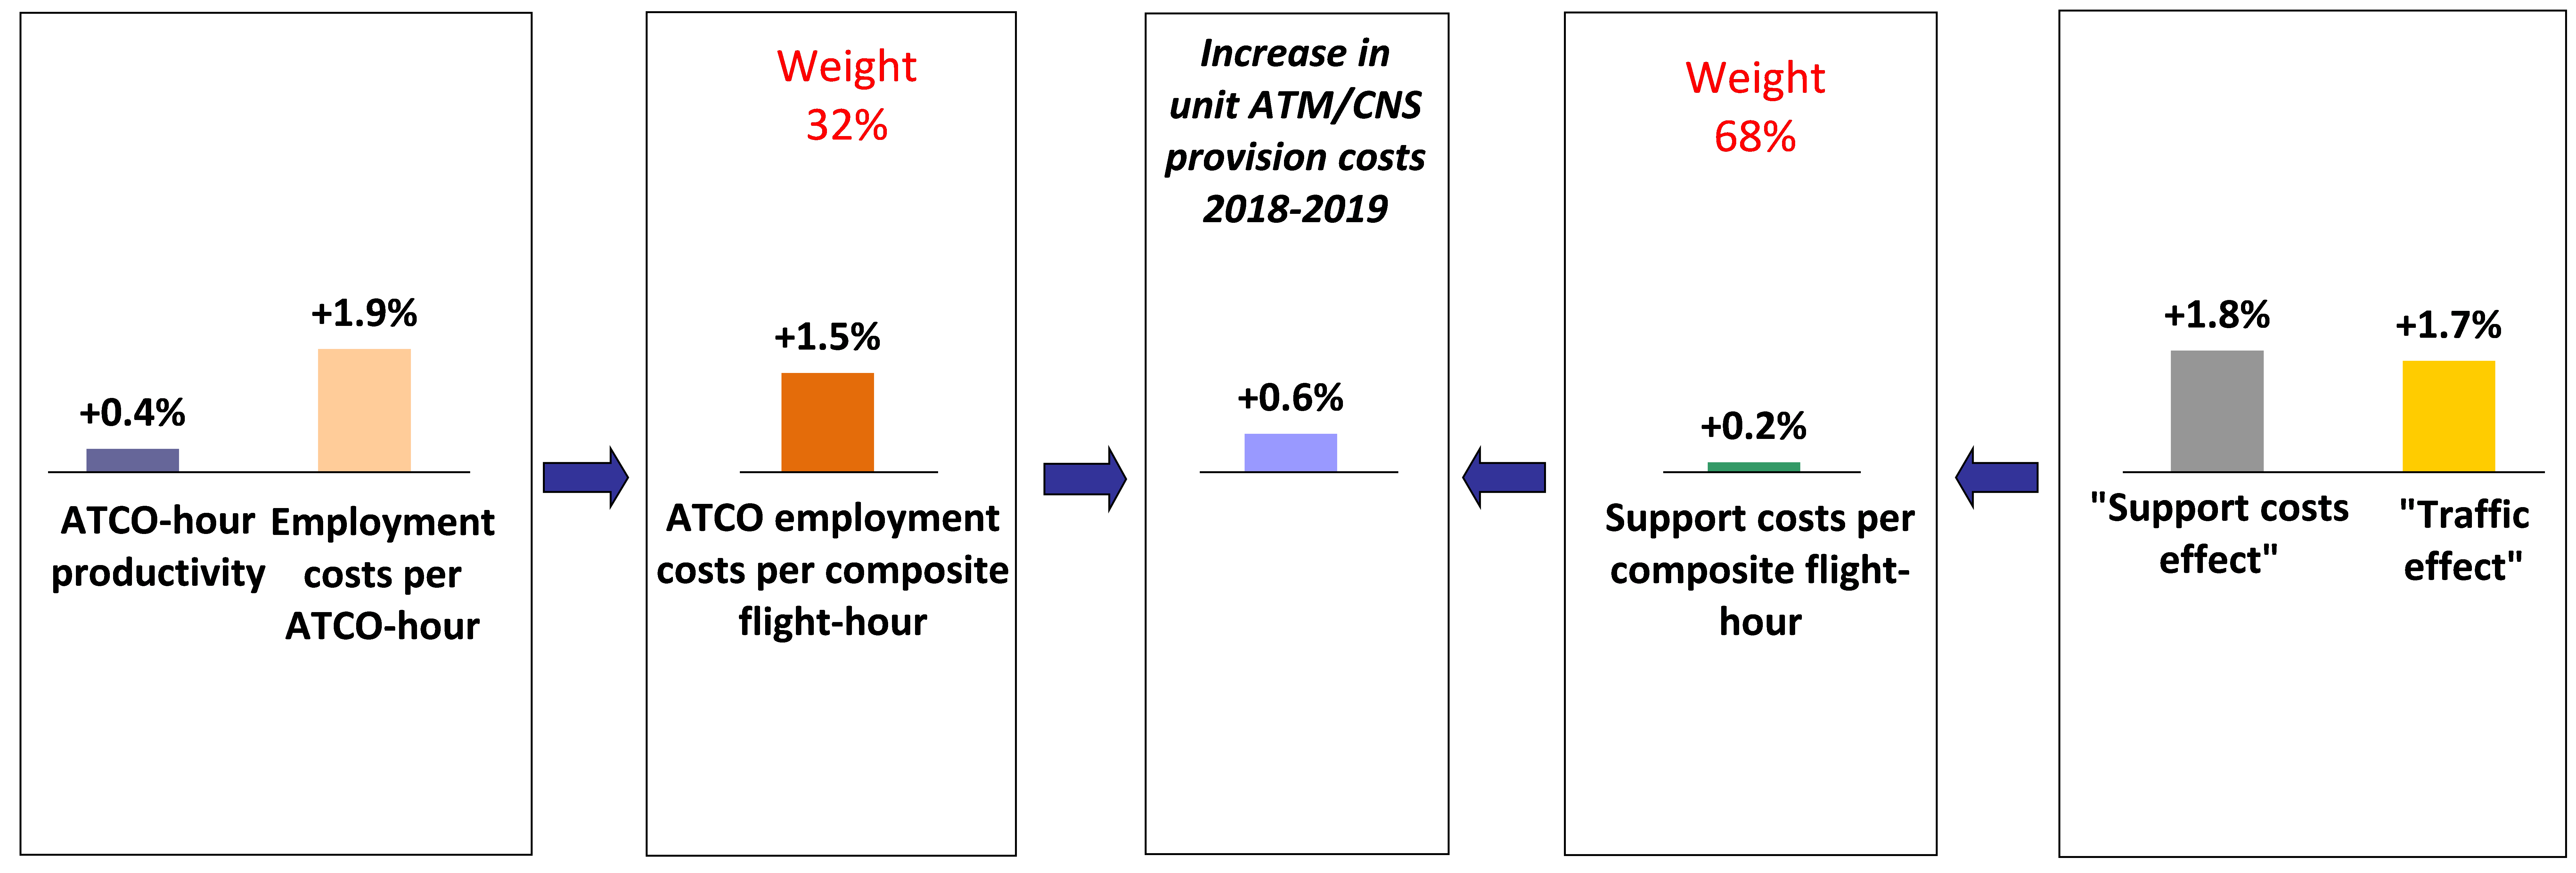
\includegraphics[width=1\linewidth]{figures/Figure 4-3} 

}

\caption{Breakdown of changes in unit ATM/CNS provision costs, 2018-2019 (real terms).}\label{fig:figure13}
\end{figure}

The two following pages provide information on the level of ATCO-hour productivity, ATCO employment costs per ATCO-hour and unit support costs for each individual ANSP.

\hypertarget{ansp-level}{%
\section{ANSP level}\label{ansp-level}}



\begin{figure}

{\centering 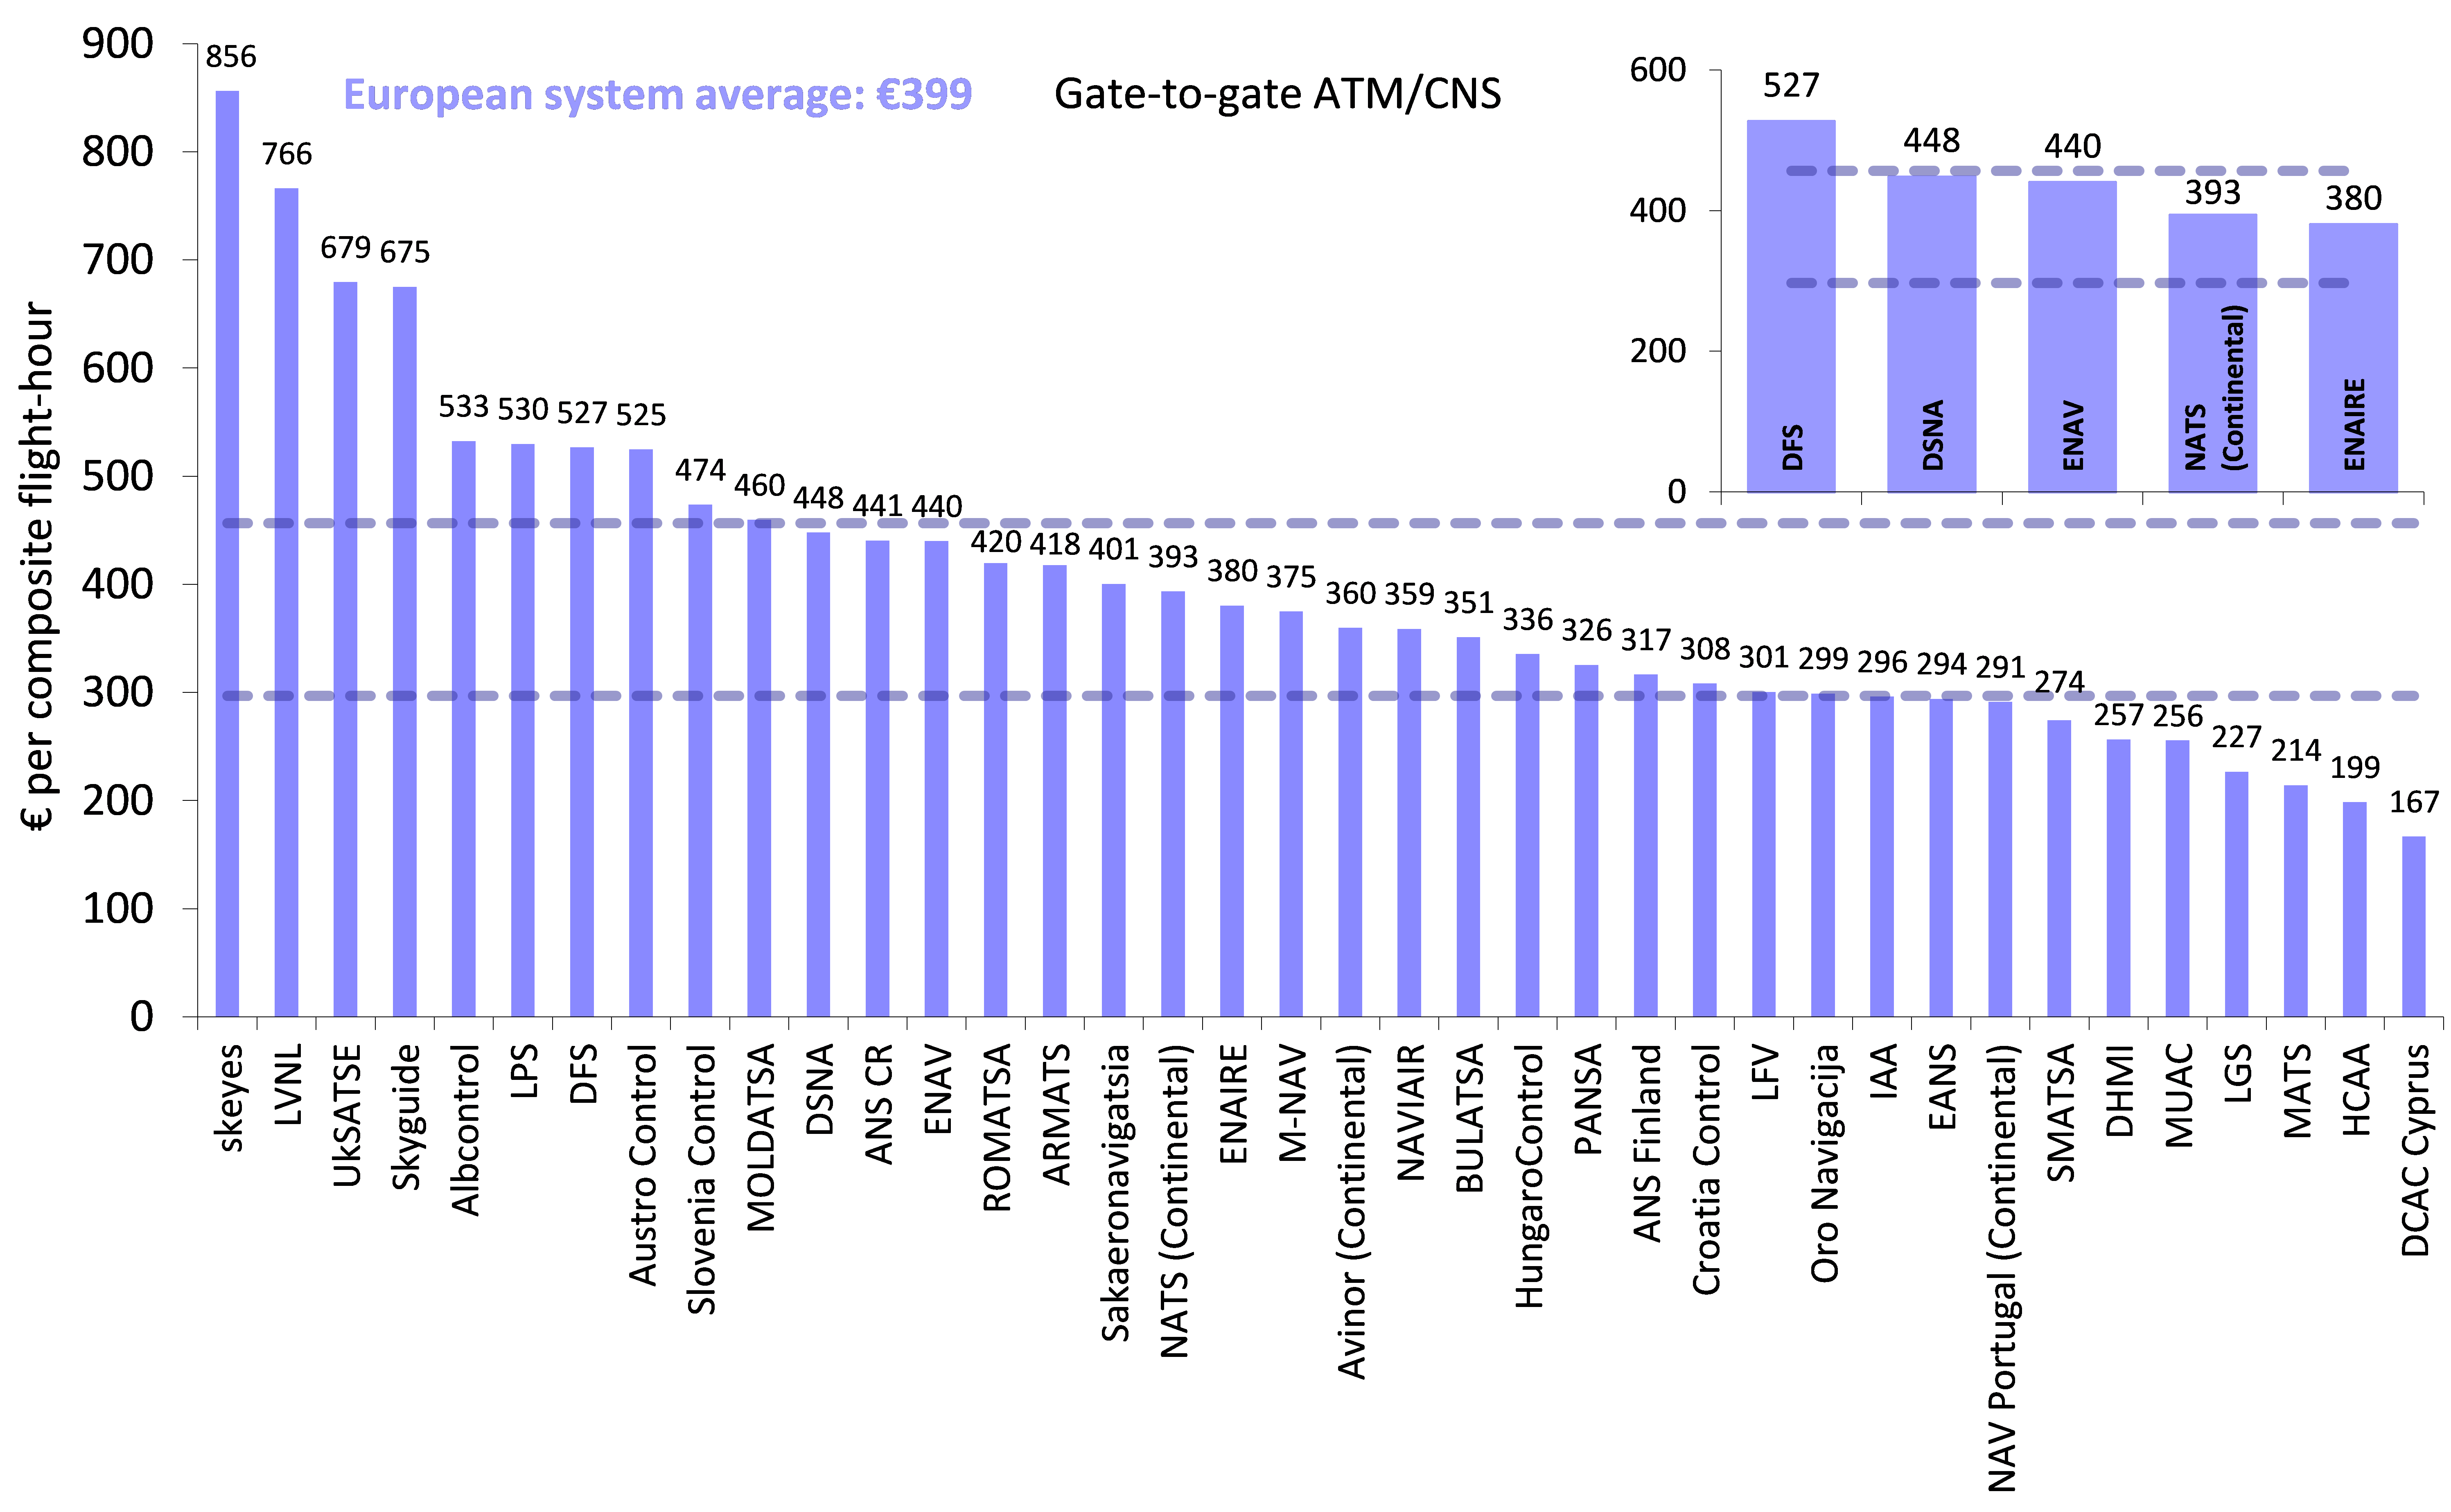
\includegraphics[width=1\linewidth]{figures/Figure 4-4} 

}

\caption{Financial gate-to-gate cost-effectiveness\footnote{For the purposes of the ACE benchmarking analysis, costs relating to ATM/CNS infrastructure shared with the military authority (€20.0M) are included in ENAIRE 2019 ATM/CNS provision costs. These costs, which are charged to civil airspace users, are not passing through ENAIRE Accounts from 2014 onwards but are borne by the Spanish Air Force (Ministry of Defence) as well as corresponding revenues. Without these costs, ENAIRE unit ATM/CNS provision costs would be slightly lower and would amount to €371.} , 2019.}\label{fig:figure14}
\end{figure}



\begin{figure}

{\centering 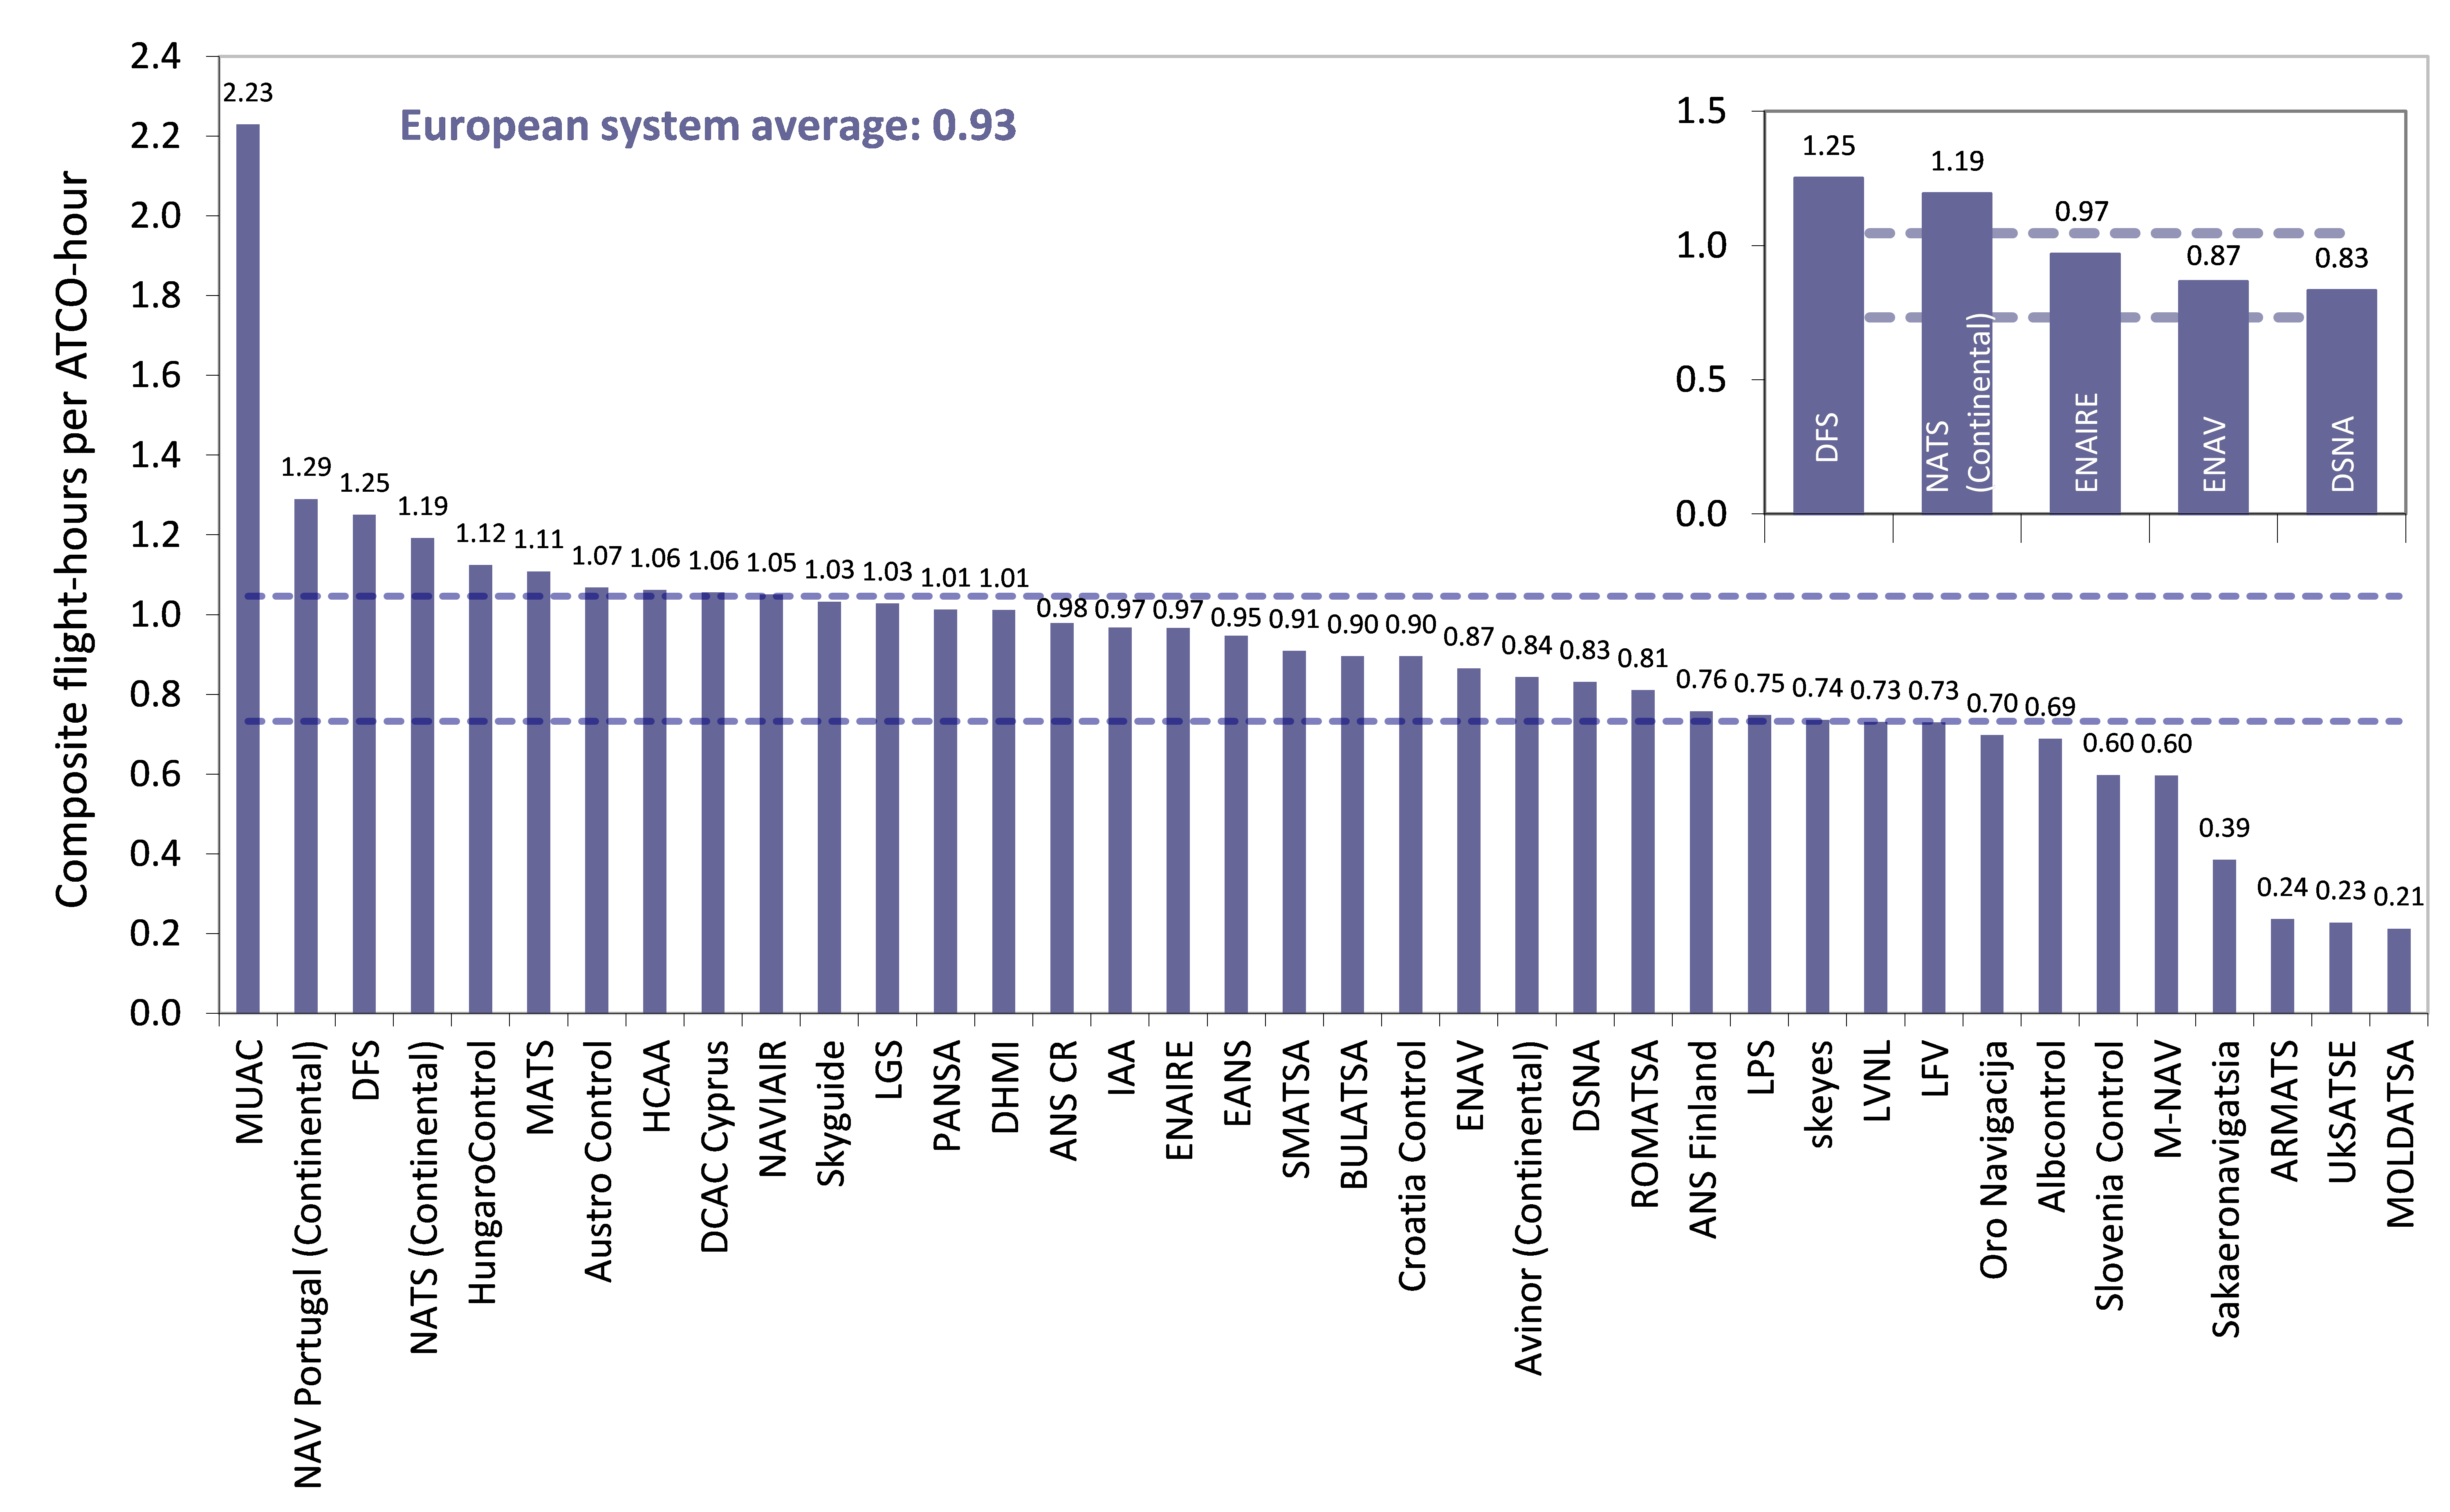
\includegraphics[width=1\linewidth]{figures/Figure 4-5} 

}

\caption{ATCO-hour productivity, 2019.}\label{fig:figure15}
\end{figure}



\begin{figure}

{\centering 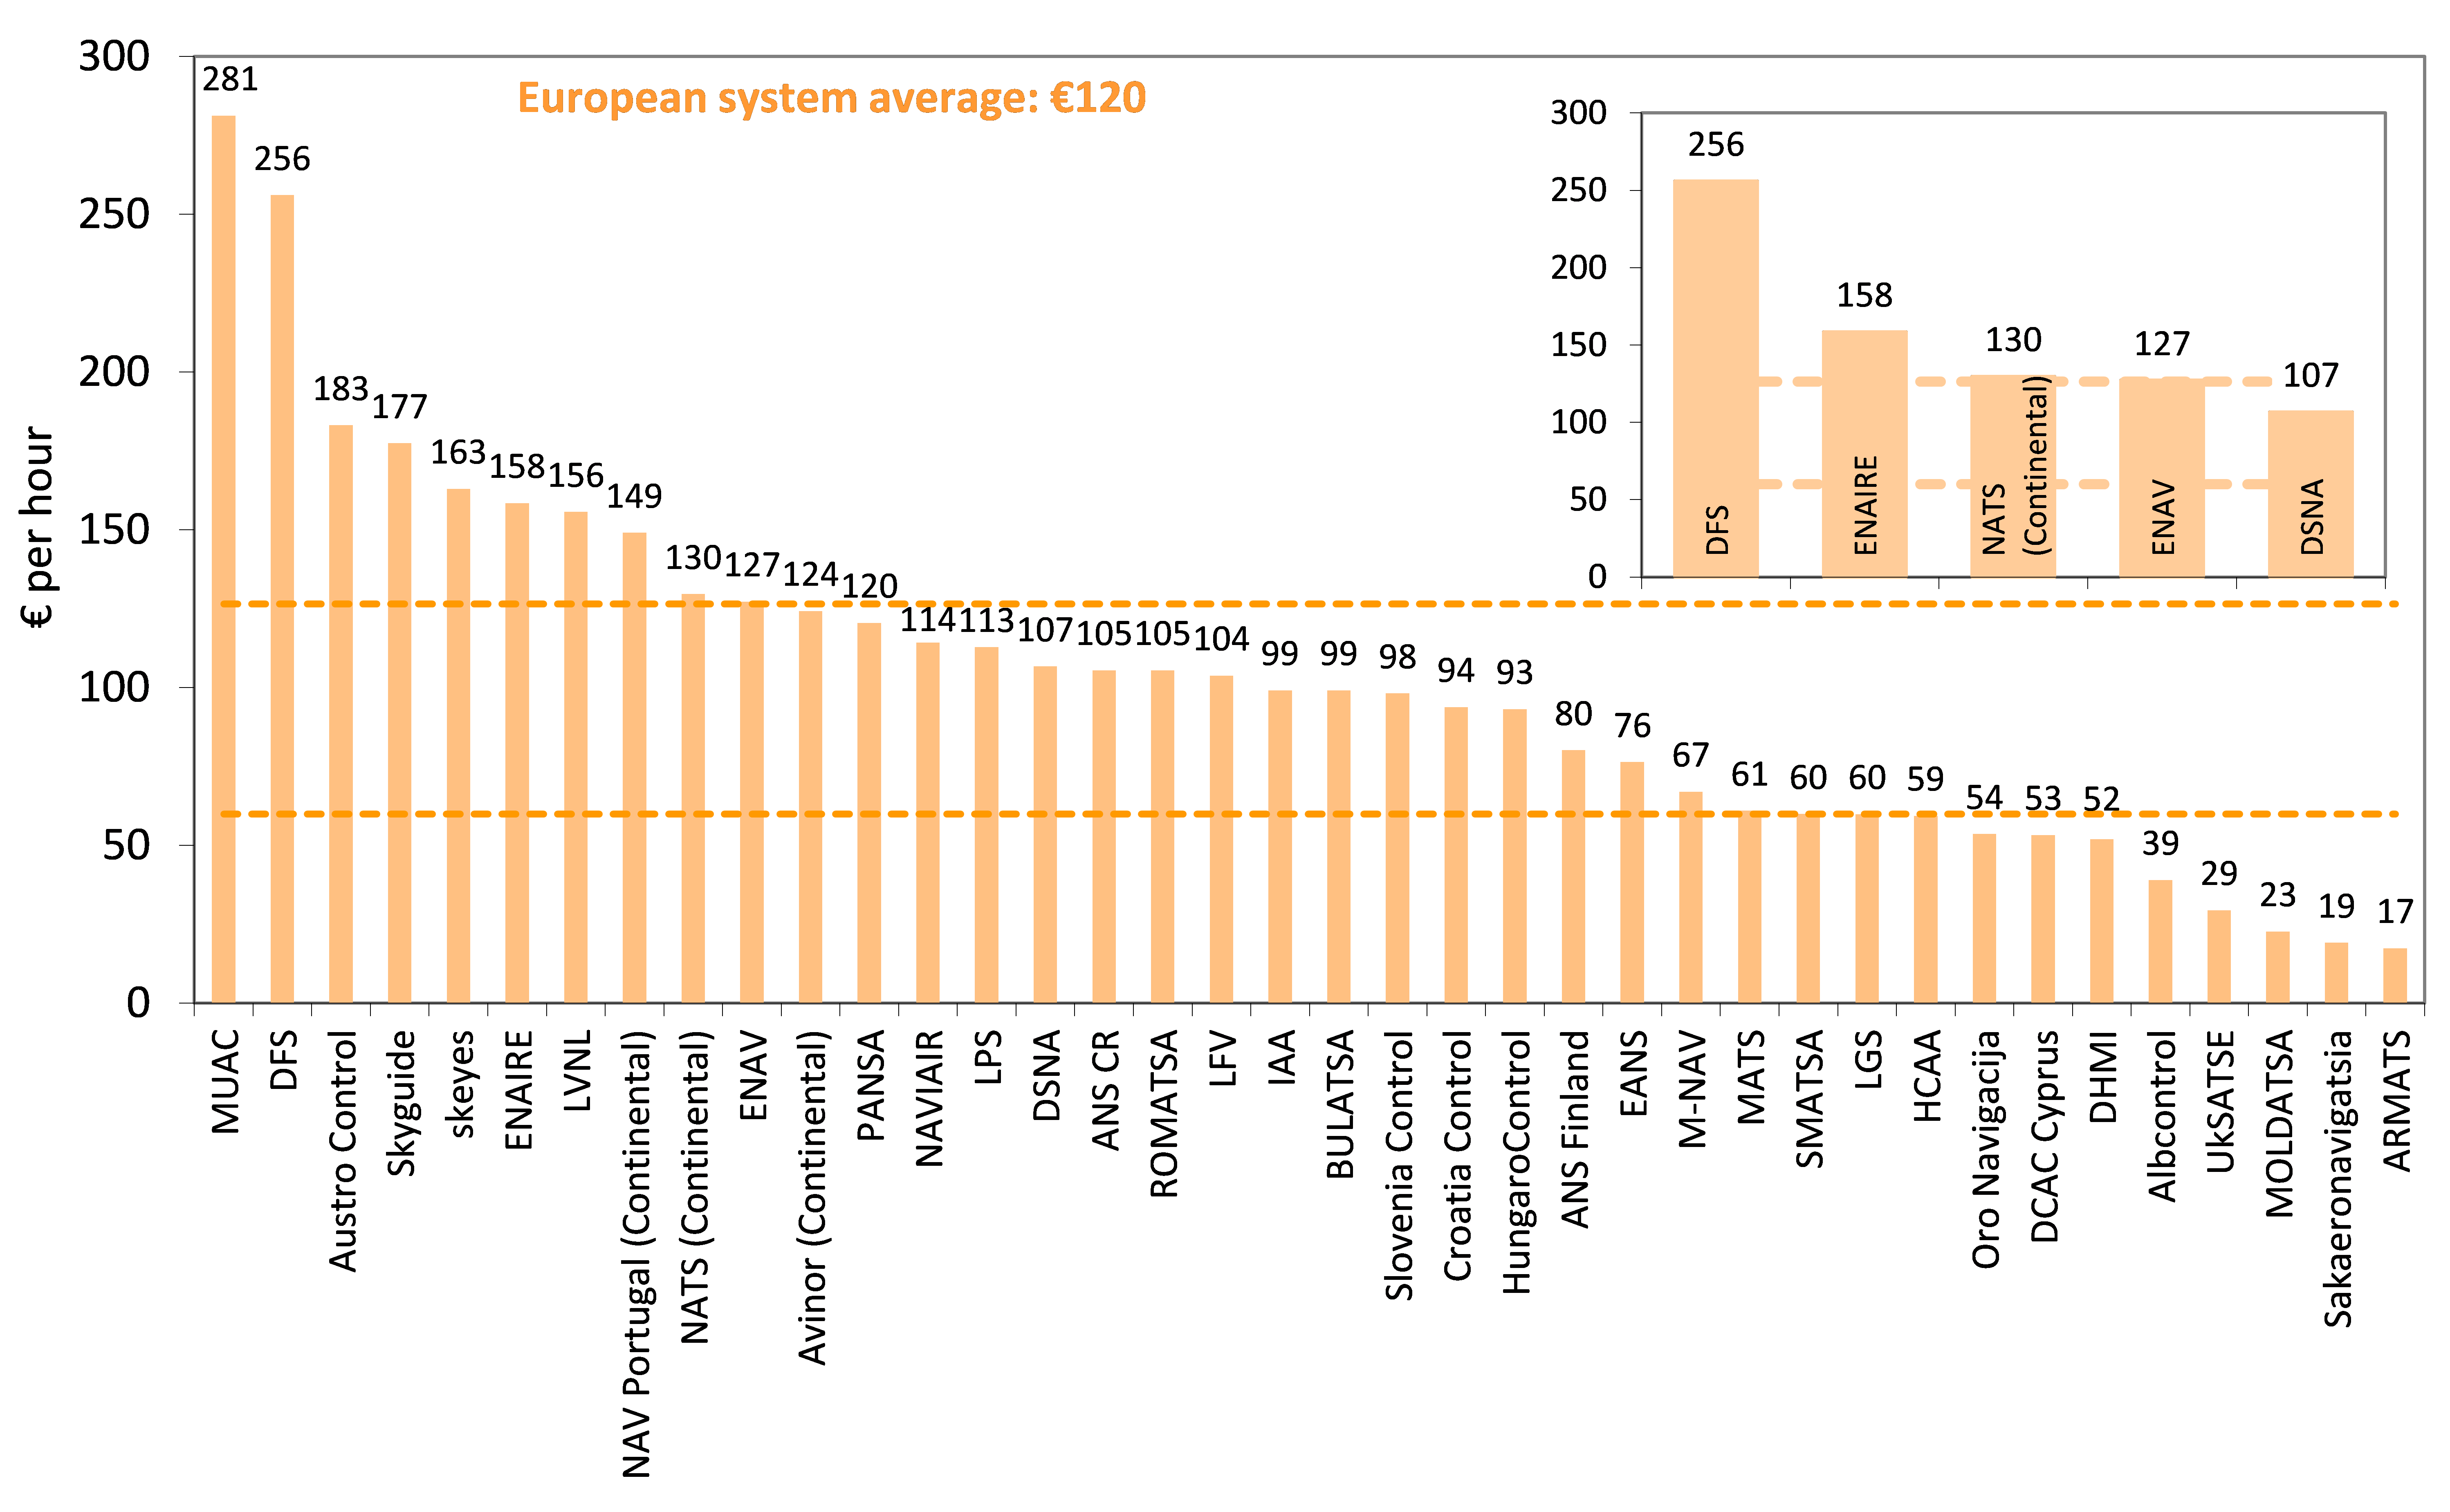
\includegraphics[width=1\linewidth]{figures/Figure 4-6} 

}

\caption{Employment costs per ATCO-hour, 2019.}\label{fig:figure16}
\end{figure}



\begin{figure}

{\centering 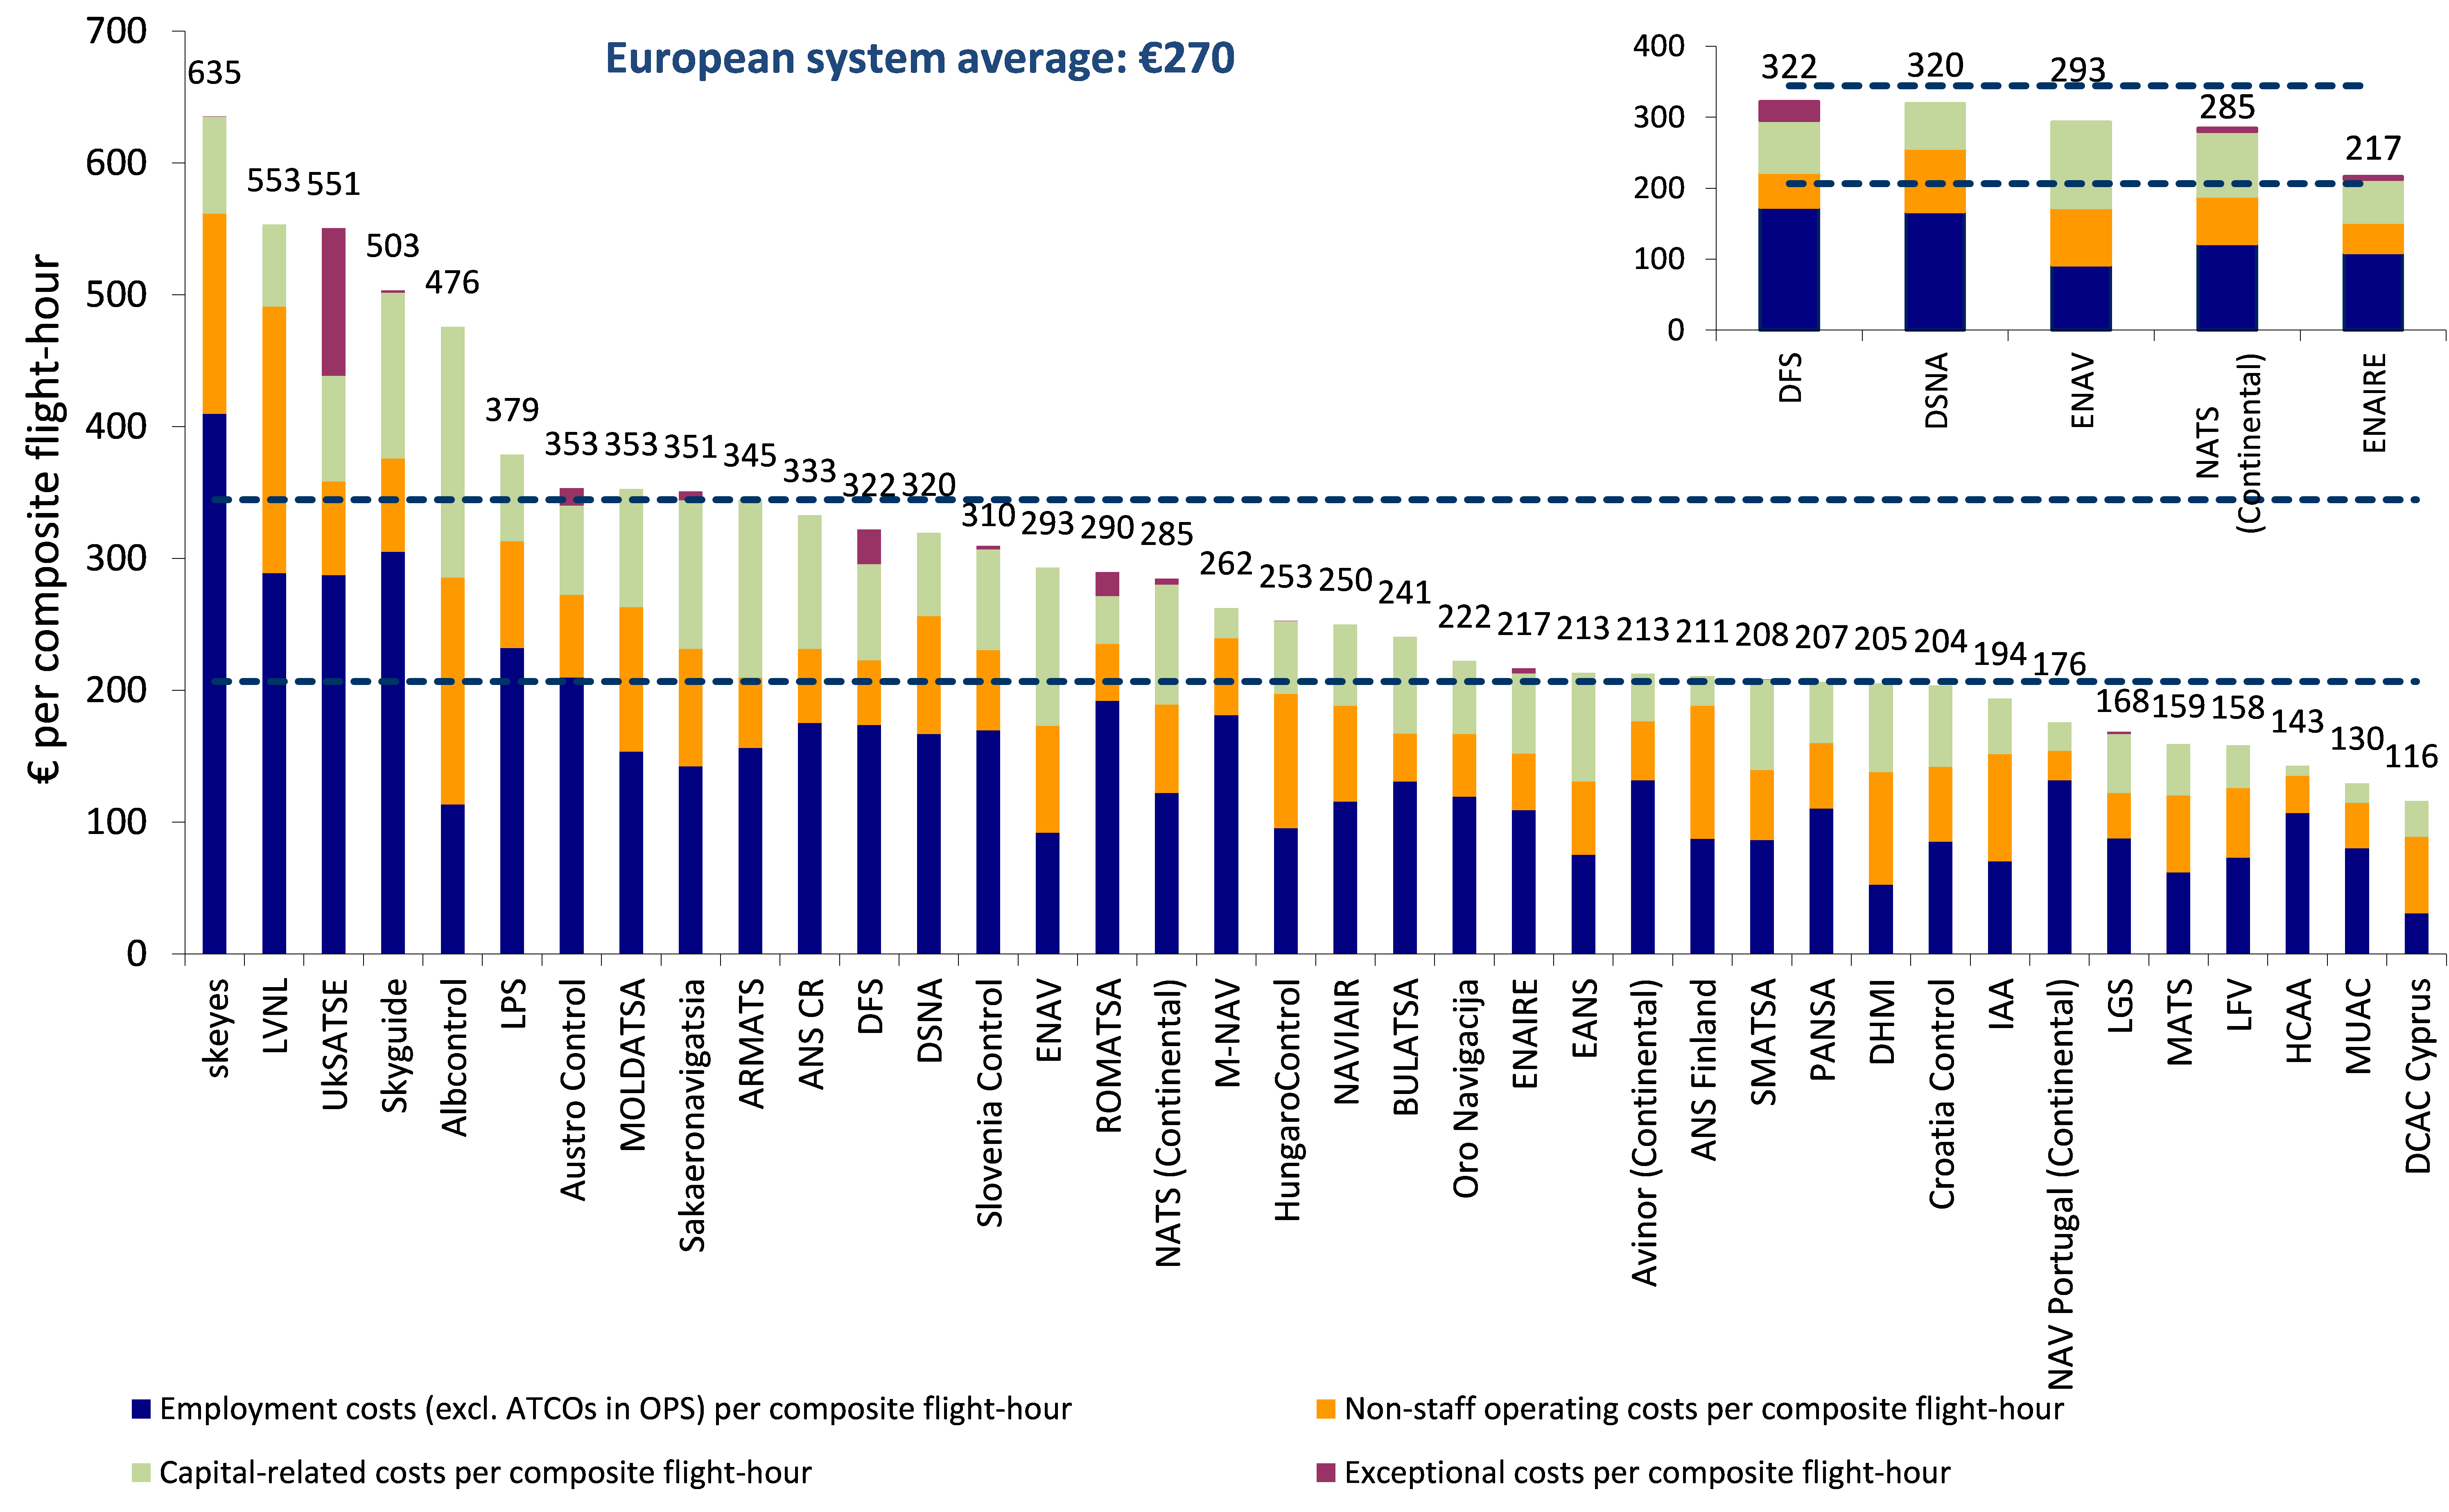
\includegraphics[width=1\linewidth]{figures/Figure 4-7} 

}

\caption{Breakdown of support costs per composite flight-hour, 2019.}\label{fig:figure17}
\end{figure}

A more detailed analysis of the changes in cost-effectiveness, ATCO-hour productivity, ATCO employment costs per ATCO-hour and unit support costs will be available in the final ACE 2019 benchmarking report.

\hypertarget{disclaimer}{%
\chapter*{Disclaimer}\label{disclaimer}}
\addcontentsline{toc}{chapter}{Disclaimer}

\begin{infobox}{caution}
\textbf{Disclaimer}

The Performance Review Unit (PRU) has made every effort to ensure that the information and analysis contained in this document are as accurate and complete as possible. Should you find any errors or inconsistencies we would be grateful if you could please bring them to the PRU's attention. The PRU's e-mail address is \href{mailto:pru-support@eurocontrol.int}{\nolinkurl{pru-support@eurocontrol.int}}

\end{infobox}

\hypertarget{r-markdown}{%
\section{R Markdown}\label{r-markdown}}

This is an R Markdown document. Markdown is a simple formatting syntax for authoring HTML, PDF, and MS Word documents. For more details on using R Markdown see \url{http://rmarkdown.rstudio.com}.

When you click the \textbf{Knit} button a document will be generated that includes both content as well as the output of any embedded R code chunks within the document. You can embed an R code chunk like this:

\begin{Shaded}
\begin{Highlighting}[]
\FunctionTok{summary}\NormalTok{(cars)}
\end{Highlighting}
\end{Shaded}

\begin{verbatim}
##      speed           dist    
##  Min.   : 4.0   Min.   :  2  
##  1st Qu.:12.0   1st Qu.: 26  
##  Median :15.0   Median : 36  
##  Mean   :15.4   Mean   : 43  
##  3rd Qu.:19.0   3rd Qu.: 56  
##  Max.   :25.0   Max.   :120
\end{verbatim}

\hypertarget{including-plots}{%
\section{Including Plots}\label{including-plots}}

You can also embed plots, for example:

\begin{center}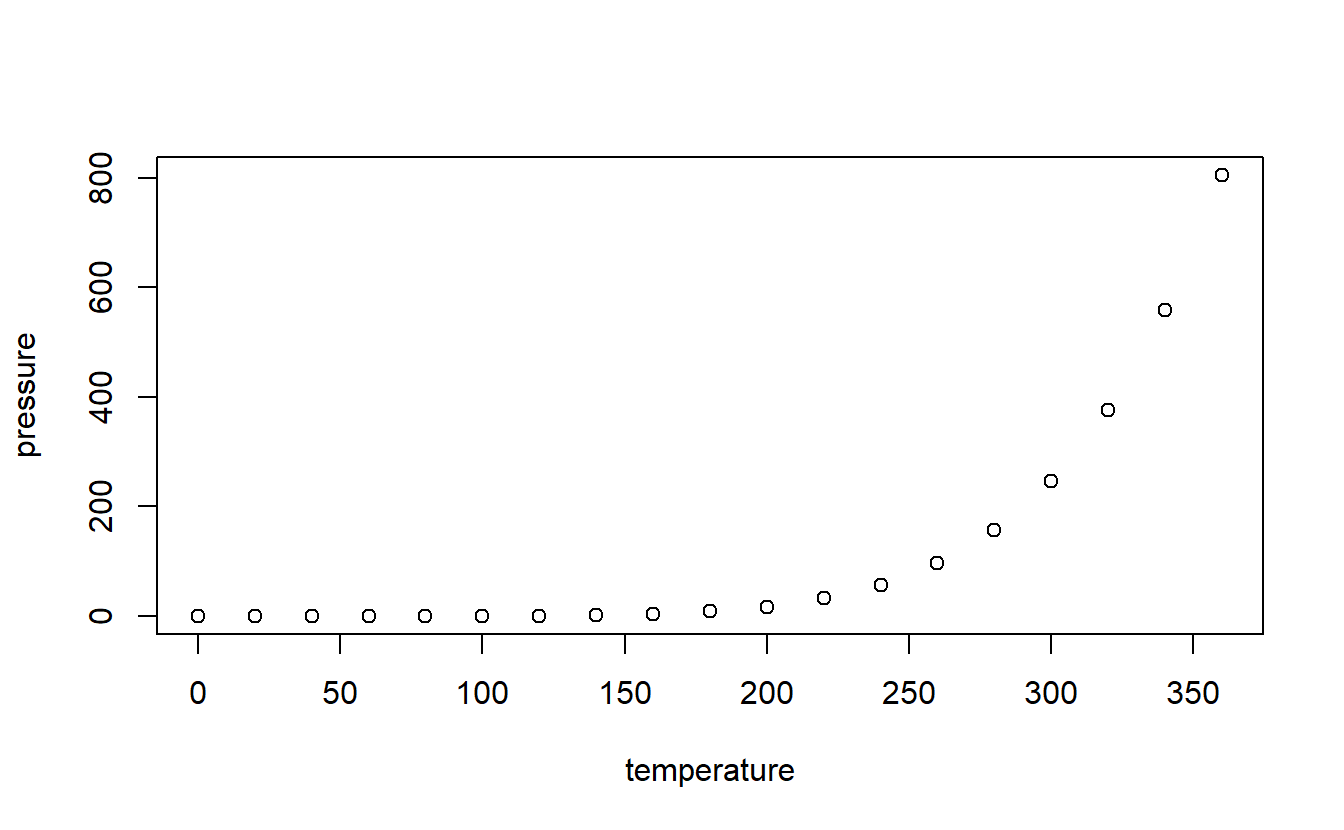
\includegraphics[width=1\linewidth]{Test_files/figure-latex/pressure-1} \end{center}

Note that the \texttt{echo\ =\ FALSE} parameter was added to the code chunk to prevent printing of the R code that generated the plot.

  \bibliography{book.bib,packages.bib}

\end{document}
